%%
%% Arquivo principal para:
%% - trabalhos de conclusão de curso
%%
%%NOTA: ESSE MODELO DE TCC FOI BASEADO NO MODELO DE TESE E DISSERTAÇÃO DO PPGEEC,
%%      DA UFRN,  COM  AUTORIZAÇÃO  DO  SEU  AUTOR, O PROFESSOR ADELARDO MEDEIROS
%%
%% Criado por Adelardo Medeiros, professor do Curso de Engenharia de Computação da UFRN, dezembro de 2005. 
%% Revisado pelos alunos de Metodologia da Pesquisa Científica de 2016.1, do curso de Engenharia de Computação da UFRN.
%% Adaptado por Diogo Henrique Duarte Bezerra, professor do Curso de Engenharia de Computação da UFMT, dezembro de 2020.

% DEFINIÇÕES GLOBAIS

% Esta primeira linha dá informações gerais sobre o documento.
% PARA A VERSÃO FINAL:
% papel A4, letra grande (12pt), openright (capítulos só iniciam em
% página direita, se necessário incluindo uma página em branco),
% twoside (o documento vai ser impresso em frente e costa)
\documentclass[a4paper,12pt,openright,twoside]{book}
% PARA A QUALIFICAÇÃO E PARA A VERSÃO INICIAL:
% papel A4, letra grande (12pt), openany (capítulos iniciam em
% qualquer página), oneside (o documento vai ser impresso só na frente)
%\documentclass[a4paper,12pt,openany,oneside]{book}

% PACOTES OBRIGATÓRIOS

% Use estes pacotes para poder digitar diretamente as letras com acento
% e para que a hifenização funcione corretamente
\usepackage[utf8]{inputenc}
\usepackage{ae}
% Para usar fontes standard ao invés das do LaTeX (gera melhores PDFs)
\renewcommand{\familydefault}{\sfdefault}
\usepackage{pslatex}
%\usepackage{helvet}
% Para a hifenização em português
\usepackage[portuges, brazil]{babel}
% Para que os primeiros parágrafos das seções também sejam indentados
\usepackage{indentfirst}
% Para poder incluir gráficos (figuras)
\usepackage{graphicx}
% Para poder fazer glossário ou lista de símbolos
% Use a segunda opção se quiser incluir na definição do símbolo a
% página e/ou a equação onde ela foi definida
\usepackage[portuguese,noprefix]{nomencl}
%\usepackage[portuguese,noprefix,refeq,refpage]{nomencl}
% Para permitir espaçamento simples, 1 1/2 e duplo
\usepackage{setspace}
% Para usar alguns comandos matemáticos avançados muito úteis
\usepackage{amsmath}
% Para poder usar o ambiente "comment"
\usepackage{verbatim}
% Para poder ter tabelas com colunas de largura auto-ajustável
\usepackage{tabularx}
% Para executar um comando depois do fim da página corrente
\usepackage{afterpage}
% Para formatar URLs (endereços da Web)
\usepackage{url}
% Para reduzir os espaços entre os ítens (itemize, enumerate, etc.)
% Este pacote não faz parte da distribuição padrão do LaTeX.
\usepackage{lib/noitemsep}
% Para as citações bibliográficas
%\usepackage[alf]{abntex2cite}
\usepackage[abbr]{lib/harvard}	% As chamadas são sempre abreviadas
%\harvardparenthesis{square}	% Colchetes nas chamadas
%\harvardyearparenthesis{round}	% Parêntesis nos anos das referências
%\renewcommand{\harvardand}{e}	% Substituir "&" por "e" nas referências
\usepackage{longtable}
% PACOTES OPCIONAIS

% Para poder incluir arquivos Postscript com cores (do Xfig, por exemplo)
\usepackage{color}
% Para ter células em tabelas que ocupam mais de uma linha
\usepackage{multirow}
% Para poder ter tabelas longas em mais de uma página
%\usepackage{longtable}
% Para poder escrever partes do texto em "n" colunas
%\usepackage{multicol}
% Se você quiser personalizar os cabeçalhos das páginas
%\usepackage{fancyheadings}
% Para incluir algoritmos e listagens de códigos
%\usepackage{listings}
% Para incluir pseudocódigos
\usepackage[portuguese, ruled, linesnumbered]{algorithm2e}
% Capítulos com títulos em um formato "decorado"
\usepackage{lib/capitulos}
% Hiperreferências dentro do texto e montagem dos links do índices dos
% para os leitores de pdf (deve ser o último pacote a ser inserido).
\usepackage[breaklinks]{hyperref}
% Referência correta de ambientes flutuantes (como figuras, tabelas e algoritmos).
\usepackage[all]{hypcap}

\usepackage[titletoc]{appendix}
\usepackage{pdfpages}

% NOVOS COMANDOS

% As definições dos novos comandos estão agrupadas no arquivo "comandos.tex"
% Esta separação é opcional: se você preferir, pode por as definições
% diretamente neste arquivo
% newcommand define novos comandos, que podem passar a ser usados da
% mesma forma que os comandos LaTeX de base.

% Implicação em fórmulas
\newcommand{\implica}{\quad\Rightarrow\quad} %Meio de linha
\newcommand{\implicafim}{\quad\Rightarrow}   %Fim de linha
\newcommand{\tende}{\rightarrow}
\newcommand{\BibTeX}{\textsc{B\hspace{-0.1em}i\hspace{-0.1em}b\hspace{-0.3em}}\TeX}

% Fração com parentesis
\newcommand{\pfrac}[2]{\left(\frac{#1}{#2}\right)}

% Transformada de Laplace e transformada Z
%\newcommand{\lapl}{\makebox[0cm][l]{\hspace{0.1em}\raisebox{0.25ex}{-}}\mathcal{L}}
\newcommand{\lapl}{\pounds}
\newcommand{\transfz}{\mathcal{Z}}

% Não aparecer o número na primeira página dos capítulos
\newcommand{\mychapter}[1]{\chapter{#1}\thispagestyle{empty}}

% Os capítulos sem número
\newcommand{\mychapterast}[1]{\chapter*{#1}\thispagestyle{empty}
\chaptermark{#1}
\afterpage{\markboth{\uppercase{#1}}{\rightmark}}
\markboth{\uppercase{#1}}{}
}

% Seções sem número
\newcommand{\mysectionast}[1]{\section*{#1}
\addcontentsline{toc}{section}{#1}
\markright{\uppercase{#1}}
}

% No tabularx, as celulas devem ser centradas verticalmente
\renewcommand{\tabularxcolumn}[1]{m{#1}}

% Células centralizadas horizontalmente no tabularx
\newcolumntype{C}{>{\centering\arraybackslash}X}

%% Abrevia figuras e tabelas
%\def\figurename{Fig.}
%\def\tablename{Tab.}


%
% As margens
%

% Direção horizontal

% Margem interna
% Nas páginas ímpares
\setlength{\oddsidemargin}{3.5cm}         % Margem real desejada
% Nas páginas pares
\setlength{\evensidemargin}{2.5cm}        % Margem real desejada
% Largura do texto
\setlength{\textwidth}{15cm}
% As margens laterais no LaTeX são sempre 1 polegada maiores do que as
% fixadas. Se foi fixada \setlength{\oddsidemargin}{3.5cm}, a margem
% real seria de 3.5+2.54=6.04cm. Para permitir que você não tenha que
% fazer esta conta, pode usar o número desejado nas linhas anteriores
% e a gente subtrai 1in nas próximas linhas
\addtolength{\oddsidemargin}{-1in}
\addtolength{\evensidemargin}{-1in}
% Note que a margem direita não é fixada diretamente:
% ela é obtida subtraindo-se os outros valores da largura da página.
% 3.5+15+x=21cm (largura A4) -> x = margem externa = 2.5cm

% Direção vertical

% Margem superior (entre o topo da folha e o cabeçalho), altura do
% cabeçalho e distância entre o fim do cabeçalho e o início do texto
\setlength{\topmargin}{2.0cm}             % Margem real desejada
\setlength{\headheight}{1.0cm}
\setlength{\headsep}{1.0cm}
% Altura do texto (sem cabeçalho e rodapé)
\setlength{\textheight}{22.7cm}
% Distância do fim do texto ao rodapé
\setlength{\footskip}{1.0cm}
% A margem superior no LaTeX é sempre 1 polegada maior do que a
% fixada. Se foi fixada \setlength{\topmargin}{2.0cm}, a margem
%real seria de 2.0+2.54=4.54cm. Para permitir que você não tenha que
% fazer esta conta, pode usar o número desejado na linha anterior
% e a gente subtrai 1in na próxima linha
\addtolength{\topmargin}{-1in}
% Note que a margem inferior não é fixada diretamente:
% ela é obtida subtraindo-se os outros valores, sem incluir o
% "footskip", da altura da página.
% 2.0+1.0+1.0+22.7+x=29.7cm (altura A4) -> x = margem inferior = 3cm

%
% O estilo das referências bibliográficas
%

\bibliographystyle{bibliografia/ppgee}

%
% O espaçamento entre linhas
%

% As páginas iniciais são sempre em espaçamento simples
\singlespacing

% Para a criação do glossário (ou lista de símbolos)
\makenomenclature

% Lista de arquivos a serem processados. Estes comandos "includeonly" são
% dispensáveis e devem obrigatoriamente ser comentados na hora de gerar o
% documento definitivo. Eles servem para compilar apenas parte do documento.
% É útil, durante a redação, para que não se tenha de compilar todo o
% documento a cada vez que se faz uma alteração. Por exemplo, se eu estou
% fazendo alterações na dedicatória e as outras partes não têm interesse no
% momento, posso incluir (descomentar) a linha "\includeonly{preambulo}"
%\includeonly{rosto}
%\includeonly{catalograficos}
%\includeonly{preambulo}
%\includeonly{resumos}
%\includeonly{introducao/introducao}
%\includeonly{estilo/estilo}
%\includeonly{matematica/matematica}
%\includeonly{figuras/figuras}
%\includeonly{conclusao/conclusao}
%\includeonly{apendice/apendice}

% Inicia o texto
\begin{document}

% Paginas iniciais (sem numeração)
\pagestyle{empty}

% Página de rosto (capa interna)
%
% ********** Página de Rosto
%

% titlepage gera páginas sem numeração
\begin{titlepage}

\begin{center}

\small

% O comando @{} no ambiente tabular x é para criar um novo delimitador
% entre colunas que não a barra vertical | que é normalmente utilizada.
% O delimitador desejado vai entre as chaves. No exemplo, não há nada,
% de modo que o delimitador é vazio. Este recurso está sendo usado para
% eliminar o espaço que geralmente existe entre as colunas
\begin{tabularx}{\linewidth}{@{}l@{}C@{}r@{}}
% A figura foi colocada dentro de um parbox para que fique verticalmente
% centralizada em relação ao resto da linha
\parbox[c]{2cm}{
\includegraphics[width=2cm]{pre-textuais/figuras/ufmt}} &
\begin{center}
\textsf{\textsc{Universidade Federal de Mato Grosso\\
Campus Universitário de Várzea Grande\\
Faculdade de Engenharia}}
\end{center} &
\parbox[c]{2cm}{
\includegraphics[width=2.75cm]{pre-textuais/figuras/faeng}}
\end{tabularx}

% O vfill é um espaço vertical que assume a máxima dimensão possível
% Os vfill's desta página foram utilizados para que o texto ocupe
% toda a folha
\vfill

\LARGE

\textbf{DRD - \textit{Dashboard of Data Reconciliation}: Desenvolvimento de uma aplicação \textit{web} de reconciliação de dados de processos industriais com recursos para análise de dados}

\vfill

\Large

\textbf{Nilton Aguiar dos Santos}

\vfill

\normalsize

Orientador: Prof. Dr. João Gustavo Coelho Pena
% Se não houver co-orientador, comente a próxima linha
% \\[2ex] Co-orientador: Prof. Dr. Beltrano Catandura do Amaral

\vfill

\hfill
\parbox{0.5\linewidth}{\textbf{%
% Descomente as opções que se aplicam ao seu caso
%Proposta de Tema para Qualificação}
Trabalho de Conclusão de Curso}
%Tese de Doutorado}
apresentado ao Curso de Engenharia de Computação da FAENG/CUVG/UFMT
%(área de concentração: Automação e Sistemas)
(área de concentração: Engenharia de Computação)
%(área de concentração: Telecomunicações)
como parte dos requisitos para obtenção do título de Bacharel
em Engenharia de Computação.}
%Doutor em Ciências.}

\vfill

\large

Cuiabá, MT, XX de XXXXXXX de 202X

\end{center}

\end{titlepage}


% Ficha catalográfica: os dados catalográficos devem ser fornecidos
% pela BCZM.
% Só são incluídos na versão final da tese ou dissertação. Não são
% incluídos nem na proposta de tema de qualificação nem na versão
% preliminar da tese ou dissertação: nestes casos, comente a próxima linha.
%
% ********** Ficha Catalográfica
%

\newpage

\begin{center}

% Aqui não se usou \vfill porque o \vfill é construído internamente com
% o comando \vspace. Espaços verticais no início da folha com \vspace
% são ignorados. Para que isto não ocorra deve-se usar o \vspace*
% \vspace*{\fill} é como se fosse um \vfill*
\vspace*{\fill}

%Divisão de Serviços Técnicos\\[1ex]
Catalogação da publicação na fonte.
UFMT / Biblioteca Central

\vspace{2ex}

\begin{tabular}{|p{0.9\linewidth}|} \hline
\\
Pereira, Fulano dos Anzóis.\\
\hspace{1em} Sobre a Preparação de Trabalho de Conclusão de Curso em Engenharia de Computação da FAENG/CUVG/UFMT /
Fulano dos Anzóis Pereira - Cuiabá, MT, 202X \\
\hspace{1em} 23 p. \\
\\
\hspace{1em} Orientador: Sicrano Matosinho de Melo \\
\hspace{1em} Co-orientador: Beltrano Catandura do Amaral \\
\\
\hspace{1em} Trabalho de Conclusão de Curso (graduação) - Universidade Federal de Mato Grosso.
Campus Universitário de Várzea Grande. Faculdade de Engenharia. Curso de Graduação em Engenharia de Computação. \\
\\
\hspace{1em} 1. Redação técnica - TCC. 2. \LaTeX - Trabalho de Conclusão de Curso.
I. Melo, Sicrano Matosinho de. II. Amaral, Beltrano Catandura do.
III. Título. \\
\\
MT/UF/BC \hfill CDU 004.932(043.2) \\ \hline
\end{tabular} 

\end{center}


% Assinaturas da banca, dedicatória e agradecimentos
% Só são incluídos na versão final da tese ou dissertação. Não são
% incluídos nem na proposta de tema de qualificação nem na versão
% preliminar da tese ou dissertação: nestes casos, comente a próxima linha.
%
% ********** Página de assinaturas
%

\begin{titlepage}

\begin{center}

\LARGE

\textbf{DRD - \textit{Dashboard of Data Reconciliation}: Desenvolvimento de uma aplicação \textit{web} de reconciliação de dados de processos industriais com recursos para análise de dados}

\vfill

\Large

\textbf{Nilton Aguiar dos Santos}

\end{center}

\vfill

% O \noindent é para eliminar a tabulação inicial que normalmente é
% colocada na primeira frase dos parágrafos
\noindent
% Descomente a opção que se aplica ao seu caso
% Note que propostas de tema de qualificação nunca têm preâmbulo.
Trabalho de Conclusão de Curso
%Tese de Doutorado
aprovado em XX de XXXXXXX de 202X pela banca examinadora composta
pelos seguintes membros:

% Os nomes dos membros da banca examinadora devem ser listados
% na seguinte ordem: orientador, co-orientador (caso haja),
% examinadores externos, examinadores internos. Dentro de uma mesma
% categoria, por ordem alfabética

\begin{center}

\vspace{1.5cm}\rule{0.95\linewidth}{1pt}
\parbox{0.9\linewidth}{%
Prof. Dr. Sicrano Matosinho de Melo (orientador) \dotfill\ FAENG/CUVG/UFMT}

\vspace{1.5cm}\rule{0.95\linewidth}{1pt}
\parbox{0.9\linewidth}{%
Prof. Dr. Beltrano Catandura do Amaral (co-orientador) \dotfill\ FAENG/CUVG/UFMT}

\vspace{1.5cm}\rule{0.95\linewidth}{1pt}
\parbox{0.9\linewidth}{%
Prof. Dr. Clint Stallone da Silva \dotfill\ IC/UFMT}

%\vspace{1.5cm}\rule{0.95\linewidth}{1pt}
%\parbox{0.9\linewidth}{%
%Profª Drª Florisbela do Amaral \dotfill\ DCA/UFRN}

\end{center}

\end{titlepage}

%
% ********** Dedicatória
%

% A dedicatória não é obrigatória. Se você tem alguém ou algo que teve
% uma importância fundamental ao longo do seu curso, pode dedicar a ele(a)
% este trabalho. Geralmente não se faz dedicatória a várias pessoas: para
% isso existe a seção de agradecimentos.
% Se não quiser dedicatória, basta excluir o texto entre
% \begin{titlepage} e \end{titlepage}

\begin{titlepage}

\vspace*{\fill}

\hfill
\begin{minipage}{0.5\linewidth}
\begin{flushright}
\large\it
``Não é o conhecimento, mas o ato de aprender.
Não a posse, mas o ato de chegar lá
Que garante o maior prazer''
(Carl Friedrich Gauss)
\end{flushright}
\end{minipage}

\vspace*{\fill}

\end{titlepage}

\chapter*{Agradecimentos}
\thispagestyle{empty}

\begin{trivlist}  \itemsep 2ex

\item Aos meus pais, José Roberto dos Santos e Teresa de Jesus de Souza Aguiar, por cada sacrifício, por cada gesto de amor, por cada exemplo de dedicação. 

\item Aos meus irmãos por acreditaram em meu potencial e caminharam ao meu lado nesta jornada acadêmica. 

\item À minha namorada por ter me motivado a cada segundo do processo.

\item Ao meu orientador, João Gustavo Coelho Pena, pela inspiração e dedicação.

\item Ao corpo docente da UFMT por todo esforço durante todo o meu curso para me dar um ótimo ensino.

\item À UFMT, pelo apoio financeiro.

\end{trivlist}


%
% O espaçamento entre linhas (ATENÇÃO A ESTA PARTE!)
%
%%%%%%%%%%%%%%%%%%%%%%%%%%%%%%%%%%%%%%%%%%%%%%%%%%%%%%%%%%%%%%%%%%%%%%%%%%%%
% PARA A VERSÃO FINAL:
% Deve ser usado espaçamento simples nas páginas de texto
%\singlespacing
% PARA A QUALIFICAÇÃO E PARA A VERSÃO INICIAL:
% Deve ser usado espaçamento 1 1/2 nas páginas de texto
\doublespacing
%%%%%%%%%%%%%%%%%%%%%%%%%%%%%%%%%%%%%%%%%%%%%%%%%%%%%%%%%%%%%%%%%%%%%%%%%%%%

% Resumo/Abstract
%
% ********** Resumo
%

% Usa-se \chapter*, e não \chapter, porque este "capítulo" não deve
% ser numerado.
% Na maioria das vezes, ao invés dos comandos LaTeX \chapter e \chapter*,
% deve-se usar as nossas versões definidas no arquivo comandos.tex,
% \mychapter e \mychapterast. Isto porque os comandos LaTeX têm um erro
% que faz com que eles sempre coloquem o número da página no rodapé na
% primeira página do capítulo, mesmo que o estilo que estejamos usando
% para numeração seja outro.
\mychapterast{Resumo}

Neste trabalho de conclusão de curso, desenvolveu-se DRD (\textit{Dashboard of Data Reconciliation}), um \textit{software online} de análise, reconciliação e qualidade de dados utilizando técnicas de minimização de funções multivariáveis pelo método dos multiplicadores de Lagrange. A solução toma como prioridade uma abordagem baseada na \textit{web}, oferecendo ao usuário a capacidade de realizar a análise e reconciliação de dados de forma remota e eficiente, com foco nos conceitos computacionais modernos afim dessa experiência ser a mais facilitada possível. Se utiliza durante todo o \textit{software} a aplicação de cálculos matemáticos e estatísticos voltados ao problema de análise, reconciliação e qualidade de dados. 
    
Por meio da ferramenta é possível modelar todo um processo industrial e alimentá-lo com os dados oriundos da planta em questão e a partir disso analisar, reconciliar e verificar a qualidade dos dados em tempo real. O \textit{software} é uma solução inovadora dado que não há um direto competidor para as funções oferecidas em um ambiente mais acessível e ágil no estado de Mato Grosso. Ao longo deste trabalho, o processo filosófico do desenvolvimento, os cálculos matemáticos, os conceitos estatísticos e computacionais, e a lógica do \textit{software} aplicada como solução são explicados de forma detalhada. Exemplos do código funcional e considerações finais sobre o trabalho realizado são apresentados nos últimos capítulos.

\vspace{1.5ex}

{\bf Palavras-chave}: Análise de Qualidade de Dados, \textit{Dashboard}, Desenvolvimento de \textit{Software}, Desenvolvimento \textit{Web}, Indústria 4.0, Multiplicadores de Lagrange, Reconciliação de Dados.

%
% ********** Abstract
%
\mychapterast{Abstract}

In this undergraduate thesis, the development of DRD (Dashboard of Data Reconciliation) was undertaken, an online software for data analysis, reconciliation, and quality assessment using techniques of multivariable function minimization through the method of Lagrange multipliers. The solution prioritizes a web-based approach, providing users with the ability to remotely and efficiently perform data analysis and reconciliation, focusing on modern computational concepts to ensure a user-friendly experience. The software applies mathematical and statistical calculations throughout, specifically tailored to the problems of data analysis, reconciliation, and quality.

Through this tool, it is possible to model an entire industrial process and feed it with data from the relevant plant, allowing real-time analysis, reconciliation, and quality verification. The software stands out as an innovative solution, as there is no direct competitor offering similar functions in a more accessible and agile environment in the state of Mato Grosso. This work details the philosophical process of development, mathematical calculations, statistical and computational concepts, and the logic of the software as an applied solution. Examples of functional code and final considerations about the work are presented in the last chapters.
\vspace{1.5ex}

{\bf Keywords}: Dashboard, Data Quality Analysis, Data Reconciliation, Industry 4.0, Lagrange Multipliers, Software Development, Web Development.


% Paginas introdutórias (com numeração romana)
\frontmatter

% Lista de conteúdo (sumário, gerado automaticamente)
% Aqui, e em todos os itens antes da introdução, o comando \phantomsection é utilizado.
% O seu uso é neecssário para auxiliar o pacote "hyperref" a fazer a referência correta
% dos links do sumário, das listas (de tabelas, figuras, algoritmos) com as páginas 
% respectivas.
% Caso seja tirado, o "hyperref" irá apontar o link do sumário para o abstract, o link
% do sumário para a lista de figuras, o link das listas de figuras para a lista de tabelas,
% e assim sucessivamente.
\phantomsection
\addcontentsline{toc}{chapter}{Sumário}
\tableofcontents

% Lista de figuras (gerada automaticamente)
\cleardoublepage
\phantomsection
\addcontentsline{toc}{chapter}{Lista de Figuras}
\listoffigures

% Lista de tabelas (gerada automaticamente)
\cleardoublepage
\phantomsection
\addcontentsline{toc}{chapter}{Lista de Tabelas}
\listoftables

% % Glossário (gerado automaticamente - veja entradas em
% % tex/00-introducao/introducao.tex e em tex/02-estilo/estilo.tex)
% \cleardoublepage
% \phantomsection
% \renewcommand{\nomname}{Lista de Símbolos e Abreviaturas}
% \markboth{\MakeUppercase{\nomname}}{\MakeUppercase{\nomname}}
% \addcontentsline{toc}{chapter}{\nomname}
% % O argumento opcional do comando \printnomenclature é a largura deixada
% % para os símbolos no glossário. Se seus símbolos são "largos", como
% % neste exemplo,  é melhor por mais espaço do que o 1cm que é reservado
% % por default
% \printnomenclature[1.5cm]

% Páginas do texto principal (com cabeçalho)
\mainmatter
\pagestyle{headings}

% Para facilitar a organização, foi criado um diretório para cada
% capítulo do documento, pois assim os arquivos das figuras ficam
% classificados por capítulos

\mychapter{Introdução}
\label{Cap:Introducao}

O setor industrial brasileiro, responsável por cerca de 20\% do PIB e 70\% das exportações \cite{cni2024}, enfrenta desafios constantes, sendo crucial para a economia nacional. A necessidade de inovação e investimentos em tecnologia apresenta ser um dos pilares da evolução do setor industrial brasileiro \cite{produtividadeindustria}. Nesse cenário, o \textit{software} de reconciliação de dados \textit{online}, denominado DRD, foi desenvolvido como uma proposta inovadora para aprimorar a qualidade e confiabilidade dos dados nos processos industriais, enquanto oferta uma interface gráfica de fácil uso e com funcionalidades de uma API (\textit{Application Programming Interface}) que permite adaptações para atender à diferentes aplicações industriais.

A precisão dos dados de processo nas indústrias químicas/petroquímicas desempenha um papel crucial no desempenho operacional e nos ganhos financeiros provenientes da utilização de diversos \textit{softwares} para monitoramento de processos, otimização \textit{online} e controle \cite{datarecshakar}. Entretanto, as medições realizadas na planta frequentemente apresentam imprecisões causadas por erros aleatórios ou sistemáticos que comprometem o modelo de processo utilizado para otimização e controle. E, para resolver problemas dessa natureza, foi desenvolvida a área de conhecimento da reconciliação de dados que faz uso de equações de processos, relações de equilíbrio e leis de conservação de massa e energia \cite{reformulationdatarecon}. De todos os possíveis métodos a serem aplicados no \textit{software} DRD, o escolhido foi o de minimização de funções multivariáveis utilizando o método dos multiplicadores de Lagrange. 

O desenvolvimento \textit{web} tem experimentado um notável crescimento na última década \cite{webusage}, e há vantagens distintas em um ambiente de \textit{software web} que não são tão prontamente acessíveis em outras áreas. As características destacáveis incluem a implementação de um sistema de API \cite{apirest}, possibilitando a interoperabilidade eficiente entre diferentes sistemas, o acesso remoto de qualquer local, a transposição fluida de ambiente de um local para outro, a facilidade inerente de manuseio \cite{apiimportance} e a capacidade natural de construção de sistemas com alta acessibilidade à indivíduos com imparidade visual. Esses atributos fazem do ambiente \textit{web} uma escolha propícia para o desenvolvimento deste sistema, proporcionando uma experiência aprimorada em comparação com alternativas menos dinâmicas, desta forma saciando uma falta do mercado como também explorando uma área não investida atualmente.

Dessa forma, é notável a necessidade de uma ferramenta que possa unificar esses dois campos, como o \textit{software} DRD. Ao integrar a teoria da reconciliação de dados com as modernas técnicas de desenvolvimento de \textit{software}, o DRD representa um avanço significativo na busca por soluções inovadoras e eficazes para os desafios enfrentados pelas indústrias. Além disso, ao aproveitar as vantagens do ambiente \textit{web}, o DRD oferece uma plataforma flexível e adaptável, capaz de atender às demandas específicas de diferentes setores industriais, promovendo assim a excelência operacional e impulsionando o desenvolvimento tecnológico do Brasil \cite{industry4status}.

\section{Objetivos}
\subsection{\textit{Objetivo geral}}

Desenvolver e implementar um \textit{software web} para a reconciliação dos dados oriundos de processos industriais, por meio do método de multiplicadores de Lagrange, visando aumentar a qualidade e a confiabilidade das informações para a análise e a tomada de decisão.

\subsection{\textit{Objetivos específicos}}

Além de buscar alcançar o objetivo principal de desenvolver uma ferramenta \textit{online} de reconciliação de dados, realizações secundárias serão contempladas, as quais serão úteis para cumprimento do objetivo alvo. Esses objetivos gerais são descritos a seguir: 

\begin{itemize}
    \item Pesquisar a respeito do estado da arte sobre as principais técnicas e ferramentas de validação, limpeza e reconciliação de dados. 
    \item Analisar e compreender as metodologias e algoritmos existentes na área de reconciliação de dados, destacando suas aplicações, vantagens e limitações. A pesquisa de estado da arte é crucial para identificar as tendências mais recentes, as melhores práticas e as lacunas existentes, proporcionando uma base sólida para o desenvolvimento da ferramenta \textit{online}.
    \item Selecionar e adaptar as tecnologias adequadas para a implementação da ferramenta \textit{online} de reconciliação de dados. Isso envolverá a avaliação de linguagens de programação, \textit{frameworks} e plataformas que melhor se adéquem aos requisitos específicos da aplicação, considerando aspectos como eficiência, escalabilidade e segurança.
    \item Projetar a arquitetura da ferramenta, delineando os componentes principais, a interação entre eles e a lógica de funcionamento. A clareza na definição da arquitetura será essencial para garantir a eficácia operacional da ferramenta, bem como para facilitar futuras atualizações e expansões.
    \item Desenvolver a ferramenta \textit{online} de reconciliação de dados, implementando os algoritmos e funcionalidades identificados na pesquisa de estado da arte. Durante essa fase, é crucial garantir a usabilidade, a integridade dos dados e a eficiência do sistema, atendendo aos padrões de qualidade e indicadores de desempenho esperados.
    \item Realizar testes abrangentes para validar a eficácia e confiabilidade da ferramenta. Isso incluirá testes de integração, testes de segurança e simulações de casos práticos para verificar a capacidade da ferramenta em lidar com diferentes cenários e volumes de dados.   
    \item Elaborar uma documentação completa, abrangendo desde o processo de desenvolvimento até as instruções de uso da ferramenta. Uma documentação completa, acessível, clara e objetiva será essencial para facilitar a compreensão, manutenção e futuras implementações relacionadas à ferramenta de reconciliação de dados.
\end{itemize}

\section{Estado da Arte}

Em meio ao processo de elaboração do trabalho de conclusão de curso, um aspecto fundamental que merece destaque é a investigação das tendências tecnológicas emergentes nas áreas relevantes para o estudo. Essa pesquisa não apenas fornece uma visão abrangente do cenário atual, mas também ajuda a identificar oportunidades para inovação e melhoria.

As tendências tecnológicas são indicadores poderosos do progresso em qualquer campo de estudo e podem ser representadas tanto na área comercial direta, como na indústria química, nas áreas adjacentes, como em conceitos de contabilidade, além de pesquisas cientificas. Elas refletem os avanços mais recentes e as direções futuras que a tecnologia pode tomar. Portanto, é essencial estar ciente dessas tendências ao realizar qualquer pesquisa acadêmica ou científica.

\subsection{Aplicação na Indústria Química}

No contexto da indústria química, há várias empresas com soluções similares à proposta neste trabalho, e a investigação das tendências tecnológicas emergentes é um aspecto crucial durante o processo de elaboração dessa ferramenta (DRD). 

\subsubsection{RECON}

A ChemPlant Technology, s.r.o, fundada em 1991 é uma empresa situada na Republica Checa, especializada em fornecer soluções tecnológicas avançadas para indústrias de processos (principalmente, processos químico, petróleo e gás, geração e distribuição de energia) \cite{reconset}. Uma de suas inovações mais notáveis é a ferramenta de reconciliação de dados chamada RECON. Esta ferramenta é fundamentada nos sólidos princípios físicos de balanço de massa e energia, um \textit{software} interativo abrangente que oferece uma plataforma robusta para modelagem de complexas plantas industriais químicas e energéticas. Ele realiza uma variedade de cálculos, incluindo balanceamento de massa, energia e momento, bem como cálculos termodinâmicos. O principal objetivo da solução é validar dados que já foram obtidos de processos operacionais. No entanto, a ferramenta, exposta na Figura \ref{fig:RECONSET} também pode ser utilizada para simular o comportamento da planta sob diferentes condições.

\begin{figure}[htbp!] 
    \begin{center}
        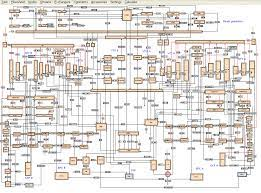
\includegraphics[width=0.75\textwidth]{figuras/RECONSET.jpg}
        \caption{Tela Principal da ferramenta RECONSET.}
        \vspace{6mm}
        \label{fig:RECONSET}
    \end{center} 
\end{figure}

O \textit{software} é orientado para PC e possui uma interface de usuário gráfica interativa, tornando-o fácil de usar. Os usuários definem problemas (ou tarefas) interativamente por meio desta interface. O RECON é capaz de equilibrar materiais e energia de componentes únicos ou múltiplos de sistemas complexos, seja em estado estacionário ou instável (dinâmico), com ou sem reações químicas (balanceamento de reatores). Além disso, ele pode realizar balanceamento de momento com base em cálculos hidráulicos de vazão em sistemas de dutos. O RECON reconcilia vazões medidas, concentrações, temperaturas e outras variáveis de processo, e calcula variáveis não medidas. Para definir um problema (ou tarefa), os usuários geralmente criam um fluxograma de processo e definem variáveis de processo, como taxas de fluxo, temperaturas, pressões, etc. O fluxograma inclui nós, fluxos de massa e energia, e trocadores de calor. Se necessário, os usuários também podem complementar (ou até mesmo substituir) o modelo de balanceamento com suas próprias equações.

\subsubsection{BILCO}

CASPEO é uma empresa francesa fundada em 2004, especializada em engenharia de processos e soluções tecnológicas. Originada do 
Departamento de Pesquisas Geológicas e Minerais da França. Ela foi criada para oferecer à indústria de mineração métodos e ferramentas computacionais resultantes de anos de pesquisa e tornou-se uma referência na indústria de processamento mineral, atendendo a vários mercados, como mineração e metalurgia, processamento de biomassa e alimentos, tratamento de resíduos sólidos e outras indústrias de processamento \cite{bilco}.

Uma das suas inovações é o \textit{software} de reconciliação de dados BILCO, projetado para derivar um balanço de material coerente e total a partir de todos os dados disponíveis (medições, análises, estimativas) para todas as correntes de processo. Ele é uma ferramenta poderosa que permite aos usuários reconciliar dados de qualquer planta de processamento, a Figura \ref{fig:BILCO}, demonstra a tela inicial do \textit{software}.

\begin{figure}[htbp!] 
    \begin{center}
        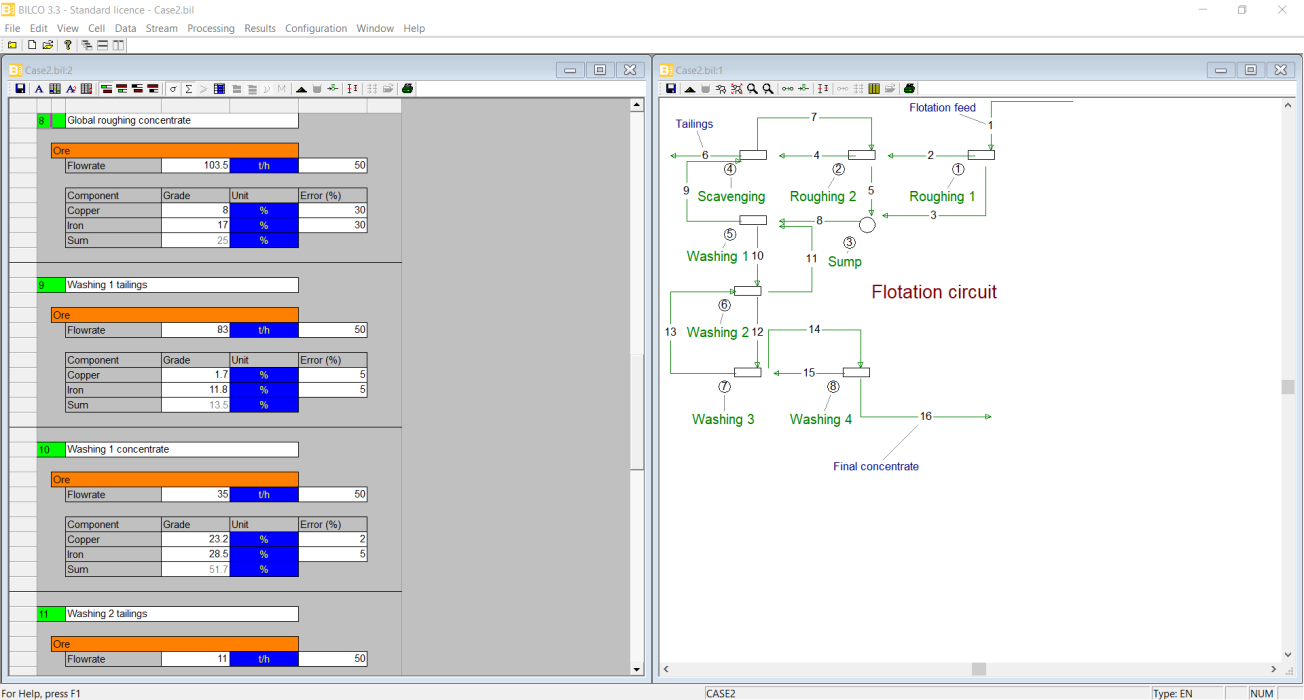
\includegraphics[width=0.75\textwidth]{figuras/BILCOCASPEOP.png}
        \caption{Tela Principal da ferramenta BILCO.}
        \vspace{6mm}
        \label{fig:BILCO}
    \end{center} 
\end{figure}

Ele tem a capacidade de se incorporar à duas outras ferramentas facilmente, no caso, à um simulador de processos, denominado USIM PAC e à um \textit{software} de contabilidade metalúrgica, INVETEO; e, dessa forma, fornece cálculos de balanço precisos e gera um conjunto de estimadores coerentes que estão em conformidades com as restrições da lei de conservação de energia, além de calcular seus erros relativos. Ele também é capaz de determinar, em quantidade e qualidade, a composição de cada corrente de processo. É um dos poucos \textit{softwares} de balanço de massa capaz de calcular toda a composição da corrente (taxas de fluxo, classes de tamanho, tipos de partículas, massa molar, etc.) em um único cálculo.

Essa solução também oferece uma única interface para gerenciar todo o processo. Consiste numa interface gráfica fácil de usar, tornando-a acessível tanto para novos usuários quanto para os mais experientes. Uma das características mais úteis do BILCO é a possibilidade de exportar os resultados para o Excel, permitindo uma análise mais profunda dos dados. Ele fornece resultados detalhados, incluindo uma planilha de comparação e uma planilha global, para uma visão completa do balanço de material.

\subsubsection{PIMSOFT}

Shorou International é uma empresa dos Emirados Árabes Unidos, que oferece soluções especializadas e serviços de engenharia com foco em automação avançada e gestão de ativos para todas as principais indústrias, com ênfase especial nos setores de petróleo, gás, utilidade e energia \cite{pimsoft}.

Uma das suas soluções é o Sistema OSIsoft PI, uma plataforma que coleta, historiza e analisa grandes quantidades de dados de séries temporais, de alta fidelidade, de várias fontes de dados e em diferentes formados. Esses dados são disponibilizados para usuários e sistemas em diversos setores de negócios. As implementações do sistema PI aproveitam o poder dos dados operacionais para gerar previsões que aumentam a consciência situacional e desencadeiam decisões bem planejadas, ajudando as empresas líderes a alcançar maiores melhorias operacionais e inovações revolucionárias em seus respectivos campos. 

E um complemento desse sistema, é o PIMSOFT SigmaFine que é um \textit{software} de verificações e balanços que utiliza princípios de conservação, estatísticas, padrões de engenharia e cálculos para monitorar e montar dados de plantas industriais. SigmaFine gera módulos coerentes, confiáveis e utilizáveis, prontos para negócios.

\subsection{Aplicação na Contabilidade}

Paralelamente à disciplina de Reconciliação de Dados na área industrial química, há uma outra área na qual investe bastante nesse campo, a de soluções contábeis. E a investigação das tendências tecnológicas emergentes é um aspecto crucial durante o processo de desenvolvimento de uma solução mais dinâmica e que consegue resolver problemas já solucionados por outras áreas da ciência.

\subsubsection{FloQast}

FloQast é uma empresa fundada em 2013, que possui uma plataforma  de contabilidade operacional baseada na nuvem, com foco em automação e gestão para uso por contadores. Uma das suas soluções é uma ferramenta de reconciliação de dados nomeada FloQast Reconciliation Management, uma solução avançada de automação de fluxo de trabalho para fornecer gerenciamento de reconciliação de contas de ponta a ponta \cite{floqast}.

Isso aumenta a velocidade e a precisão financeira do fechamento financeiro, ao mesmo tempo que gerencia o risco de declaração incorreta. Esse \textit{software} permite que controladores e suas equipes automatizem e gerenciem o processo de reconciliação de ponta a ponta, com uma solução centralizada confiável por contadores e auditores em todo o mundo.

\subsubsection{Aspen}

AspenTech, uma empresa fundada em 1981, a partir do Projeto ASPEN - uma pesquisa conjunta entre o MIT (Instituto de Tecnologia de Massachusetts) e o Departamento de Energia dos EUA na qual desenvolveu a primeira tecnologia de modelagem e simulação baseada em computador para a indústria química. Hoje, mais de 40 anos depois, com mais de 3700 funcionários e 60 localidades em todo o mundo, a empresa tem seu foco em soluções industriais, ao mesmo tempo em que enfrenta diretamente a sustentabilidade, com foco na eficiência dos recursos, transição energética, descarbonização e redução de resíduos \cite{aspen}.

Uma das suas ferramentas que utiliza soluções similares às do trabalho de conclusão de curso é a ferramenta AURA (Aspen Unified Reconciliation Accounting) uma solução que ajuda a reduzir perdas de material e aumentar margens por meio de um equilíbrio eficiente de massa e volume. Capacitando as partes interessadas a tomar melhores decisões com base em dados de produção validados e reconciliados. Sua arquitetura escalável reduz o custo total de propriedade com opções rápidas de implantação na nuvem e fácil implementação e manutenção do modelo. A precisão da reconciliação é aumentada pelo \textit{Smart Solver} proprietário que resolve automaticamente os erros de densidade medidos em laboratório. O \textit{software} também ajuda a atingir metas de redução de emissões ao automatizar o rastreamento, monitoramento e relatórios de emissões de gases de efeito estufa e intensidade de carbono do produto. Além disso, permite fechar o balanço mais rapidamente com fluxos de trabalho intuitivos, interpretação fácil dos resultados com visualização avançada e relatórios dinâmicos poderosos.

\subsection{Pesquisas Sendo Desenvolvidas}

Como o objetivo do DRD é ser uma ferramenta que consegue recolher avanços tecnológicos de cada área, é de suma importância não só estar ciente e alinhado às tendências da própria área de aplicação, como das adjacentes, mas também estar alinhado às pesquisas da área de reconciliação de dados computacional. 

\subsubsection{Controle e Supervisão de Processamento Mineral}

A pesquisa apresentada por Daniel Hoduin, \cite{danielhoduin}, dá  ênfase às restrições de conservação de massa e energia, que são usadas como base para o projeto de estratégias de medição, atualização do valor medido por técnicas de filtragem de erros de medição e estimativa de variáveis de processo não medidas. Como as principais variáveis numa unidade de processamento mineral são geralmente vazões e concentrações, a sua reconciliação com as leis de conservação de massa é central para as técnicas discutidas. São propostas ferramentas para três tipos diferentes de regimes operacionais: regime estacionário, estacionário e dinâmico. Esses métodos de reconciliação são baseados nos mínimos quadrados usuais e nas técnicas de filtragem de Kalman.

\subsubsection{Balanços de Materiais em Rede de Distribuição de Gás}

O desenvolvimento feito pelos pesquisadores Jesús David Badillo Herrera, Arlex Chaves e José Augusto Fuentes Osorio \cite{balancecontrol}, oferece uma solução prática para lidar com os desafios apresentados por erros em sistemas de distribuição de gás natural. Ao combinar técnicas numéricas e estatísticas, como a Reconciliação de Dados (DR) e a Detecção de Erros Brutos (GED), a ferramenta visa aprimorar a precisão das medições, garantir conformidade com as leis de conservação de massa e identificar e corrigir erros grosseiros. A validação da ferramenta por meio de problemas da literatura e sua aplicação a uma rede de distribuição real demonstram sua eficácia em fornecer resultados reconciliados precisos. Essa ferramenta tem o potencial de aprimorar a eficiência e confiabilidade dos processos de distribuição de gás natural, minimizando perdas de receita e complicações legais.

\section{Justificativa}

A construção do projeto de \textit{software} DRD é fundamentada na urgente necessidade de soluções inovadoras para superar os desafios do setor industrial brasileiro. Este setor é essencial para a economia do país, apesar dos constantes obstáculos que enfrenta. Destaca-se, portanto, a importância da inovação e do investimento em tecnologia como motores do seu desenvolvimento.

Além disso, a escolha de desenvolver o \textit{software} como uma aplicação \textit{web} aproveita as vantagens desse ambiente, incluindo interoperabilidade eficiente entre sistemas, acesso remoto, facilidade de uso e alta acessibilidade para indivíduos com necessidades especiais, não apenas atendendo às demandas do mercado atual, mas também representa uma inovação ao explorar uma área ainda não totalmente investida. A importância desse projeto é ainda mais destacada pela análise das tendências tecnológicas emergentes em áreas relevantes, como a indústria química. Empresas e pesquisadores estão desenvolvendo ferramentas e técnicas semelhantes, demonstrando a relevância e a demanda por soluções que otimizem a reconciliação de dados e garantam a precisão das informações.

Portanto, a solução visa preencher uma lacuna no mercado brasileiro, oferecendo uma ferramenta inovadora e eficaz para reconciliação de dados industriais. Ao integrar teoria e prática, o DRD tem o potencial de impulsionar a excelência operacional e promover o desenvolvimento tecnológico do país, contribuindo para o aumento da competitividade das indústrias brasileiras no cenário global.

O trabalho aqui apresentado é organizado da seguinte forma: no Capítulo 1 é feita a introdução do trabalho, apresentando o problema e seu contexto, citando sua solução de forma delimitada e com os objetivos principal e secundário de forma clara, e fazendo uma revisão bibliográfica sobre ferramentas que possuem alguma semelhança com a ferramenta aqui proposta; no Capítulo 2 é apresentado o referencial teórico que trás definições, descrições e detalhes sobre as principais teorias que embasam a solução proposta; o Capítulo 3 descreve como os diferentes métodos e técnicas corroboram para o êxito da solução aqui planejada e também é apresentado um cronograma de atividades, por meio do diagrama Gantt, que será útil para o organização e gerenciamento do desenvolvimento das etapas para realização da solução aqui proposta quanto no trabalho de conclusão de curso 2; por fim, no Capítulo 4 são realizadas considerações finais acerca do aprendizado com a realização deste trabalho, acerca das reflexões e ponderações sobre as expectativas de resultados para o desenvolvimento futuro do TCC2 e também sobre as contribuições desta obra.
\mychapter{Referencial Teórico}
\label{Cap:ReferencialTeorico}

Este capítulo aborda a prática da reconciliação de dados, fundamental para garantir a consistência e precisão das informações coletadas em diferentes contextos científicos e industriais e utilizada como base no desenvolvimento do \textit{software}. É detalhada sua definição, evolução e aplicação na indústria, destacando sua contribuição para a otimização de processos e a análise proativa. 
    
Além disso, é discutido o método dos multiplicadores de Lagrange como uma abordagem matemática eficaz para resolver problemas complexos de reconciliação de dados. Por fim, a sinergia entre a indústria e a internet é contextualizada, evidenciando o papel crucial do \textit{software} na atualidade.

\section{Reconciliação de Dados}
\subsection{Definição}

A reconciliação de dados é uma prática de tratamento de dados em diversos campos da ciência e da engenharia, visando garantir a consistência e a precisão dos dados coletados a partir de diferentes fontes \cite{datarecshakar}. Em sua essência, a reconciliação de dados consiste no processo de comparar e corrigir dados divergentes ou inconsistentes, a fim de garantir que todas as informações disponíveis estejam alinhadas e concordantes. Esse processo é essencial em contextos nos quais múltiplas fontes de dados são utilizadas, como em sistemas industriais, processos químicos, redes de sensores e modelagem ambiental \cite{datarecshakar}.
        
A reconciliação de dados envolve a aplicação de técnicas estatísticas e matemáticas para identificar e corrigir discrepâncias entre os dados observados e os valores esperados, com base em modelos e relações conhecidas \cite{datarecragnoli}. Isso pode incluir a detecção e correção de erros sistemáticos ou aleatórios, a estimativa de valores ausentes e a harmonização de diferentes tipos de dados. Ao garantir a consistência e a confiabilidade dos dados, a reconciliação de dados permite uma análise mais precisa e uma tomada de decisão mais fundamentada em uma variedade de contextos aplicados \cite{datarecragnoli}.
    
Em suma, a reconciliação de dados desempenha um papel crucial na garantia da qualidade e integridade dos dados em diferentes áreas de aplicação. Ao alinhar e corrigir dados discrepantes, essa prática permite uma análise mais confiável e uma interpretação mais precisa dos fenômenos estudados, contribuindo assim para avanços significativos em diversos campos da ciência e da engenharia \cite{datarecshakar}.
    
\subsection{Reconciliação de Dados no âmbito Industrial}
    
No começo da década de 1960 se entendeu a importância do controle de processos químicos industriais por computadores que aplicavam técnicas matemáticas \cite{computecontrol}, dessa forma surge a área da computação voltada à reconciliação de dados, na qual há a comparação, validação e correção de informações coletadas em diferentes pontos do processo, a fim de determinar a consistência dos dados, a qualidade dos mesmos ou até otimizar os processos \cite{datarecshakar}.
    
Ao longo das últimas décadas, os métodos de reconciliação de dados evoluíram significativamente, acompanhando os avanços tecnológicos e as demandas crescentes da indústria \cite{datarecsurvey}. Com o advento de sistemas de automação mais avançados, sensores inteligentes e a proliferação de dispositivos conectados, a quantidade de dados gerados nas operações industriais aumentou drasticamente \cite{datarecsurvey}. Nesse contexto, a reconciliação, análise e gestão de dados tornaram-se ferramentas indispensáveis para garantir a integridade e a confiabilidade das informações coletadas em tempo real \cite{aularecon}.
    
Na era contemporânea, a reconciliação de dados desempenha um papel crucial na otimização dos processos industriais, contribuindo para a eficiência operacional e a redução de custos. Sistemas avançados de reconciliação não apenas comparam e validam dados, mas também utilizam algoritmos sofisticados para identificar padrões, tendências e anomalias \cite{datarecragnoli}. Essa capacidade analítica permite que as indústrias ajam proativamente, antecipando-se a problemas potenciais, otimizando a produção e melhorando a qualidade dos produtos finais \cite{datarecshakar}.

\subsection{Reconciliação de Dados Pelo Método dos Multiplicadores de Lagrange}
    
No sistema em questão, a reconciliação de dados vai ser feita com a minimização de funções multivariáveis utilizando o método dos multiplicadores de Lagrange, desenvolvido pelo matemático Joseph Louis Lagrange (1739-1813), que desenvolveu um método de encontrar o mínimo ou máximo de uma função multivariável sujeita a uma ou várias condições de restrição \cite{lagrangebio}.
    
Nesse contexto, a aplicação do método dos multiplicadores de Lagrange destaca-se como uma abordagem matemática sofisticada e eficaz para resolver problemas complexos de reconciliação de dados \cite{optimizationlagrange}. A técnica proporciona uma estrutura robusta para lidar com situações em que é necessário otimizar uma função multivariável sujeita a restrições específicas. Ao utilizar os multiplicadores de Lagrange, o sistema ganha a capacidade de encontrar soluções que atendam simultaneamente às condições impostas, proporcionando uma reconciliação precisa e eficiente dos dados envolvidos \cite{aularecon}. Essa metodologia, fundamentada em princípios matemáticos sólidos, contribui para aprimorar a qualidade e a confiabilidade dos resultados obtidos, tornando-a uma ferramenta valiosa para a solução proposta no trabalhos.
        
\section{Desenvolvimento de um \textit{Software Online}}
\subsection{Desenvolvimento \textit{Front-End}}
    
A interface de usuário de um \textit{software}, também denominada de \textit{front-end}, desempenha um papel crucial no desenvolvimento de sistemas modernos \cite{eloquentjavascript}. É responsável por criar a experiência do usuário, tornando a interação com o \textit{software} intuitiva, eficiente e agradável. Compreende todos os elementos visíveis e interativos de uma aplicação, como botões, menus, formulários e \textit{layouts}, que são projetados e desenvolvidos para fornecer uma interface acessível e funcional aos usuários \cite{frontendperfomance}.
    
As principais tecnologias aplicadas a essa área dentro do desenvolvimento \textit{web} são linguagens de programação como HTML, CSS, JavaScript e TypeScript \cite{webdevlang}. Essas tecnologias permitem aos desenvolvedores criar interfaces de usuário dinâmicas e responsivas, capazes de se adaptar a diferentes dispositivos e tamanhos de tela. Além disso, o \textit{front-end} envolve a utilização de \textit{frameworks}, \textit{runtimes} e bibliotecas importantes e poderosas, como React, Angular e Vue.js, possibilitando um desenvolvimento rápido e eficiente de interfaces de usuário modernas \cite{frontendperfomance}. Desta forma, o \textit{front-end} é uma parte essencial do processo de desenvolvimento de \textit{software}, desempenhando um papel fundamental na criação de sistemas interativos e centrados na experiência do usuário \cite{reactjs}.

\subsection{Desenvolvimento \textit{Back-End}}
    
Muitas vezes referido como a parte não visível ou o "cérebro" por trás de uma aplicação, o \textit{back-end} é igualmente crucial para o funcionamento de sistemas modernos \cite{backend}. Enquanto o \textit{front-end} é responsável pela parte visual e interativa da aplicação, o \textit{back-end} lida com a lógica de negócios, o armazenamento de dados e a comunicação com o servidor. Isso inclui operações como autenticação de usuários, processamento de dados, gerenciamento de sessões e acesso a banco de dados \cite{backenddevroles}.
    
As tecnologias empregadas no \textit{back-end} são diversas, incluido linguagens de programação como Python, Ruby, Java, PHP e Node.js. Estas linguagens são utilizadas em conjunto com \textit{frameworks} e bibliotecas específicas para o desenvolvimento \textit{web}, como Django, Ruby on Rails, Spring, Laravel e Express.js \cite{eloquentjavascript}. O \textit{back-end} também envolve a criação de APIs (Interfaces de Programação de Aplicativos) para permitir a comunicação eficiente entre o \textit{front-end}, outros sistemas e o banco de dados. Desta forma, o \textit{back-end} é responsável por garantir que a aplicação \textit{web} seja funcional, segura e capaz de processar grandes volumes de dados, desempenhando um papel crucial no sucesso de sistemas \textit{web} modernos \cite{javascriptframework}.
    
\subsection{Desenvolvimento de Banco de Dados}
    
No contexto do desenvolvimento de sistemas \textit{web}, o banco de dados desempenha um papel fundamental na organização e armazenamento de dados utilizados pela aplicação \cite{databasedepth}. Ele oferece uma estrutura organizada e eficiente para armazenar informações de forma persistente, garantindo que os dados sejam recuperados de maneira rápida e precisa, quando necessário. O banco de dados é responsável por gerenciar grandes volumes de dados, lidar com transações complexas e garantir a integridade e a segurança das informações armazenadas \cite{databasesql}.
    
Existem diversos tipos de bancos de dados, cada um com suas características e funcionalidades específicas. Os bancos de dados relacionais, como MySQL, PostgreSQL e SQL Server, utilizam tabelas para organizar os dados em linhas e colunas, facilitando consultas complexas e garantindo a consistência dos dados por meio de relações definidas \cite{databasesqlnet}. Por outro lado, os bancos de dados NoSQL, como MongoDB e Cassandra, oferecem uma abordagem mais flexível e escalável para o armazenamento de dados não estruturados, como documentos, gráficos e dados em tempo real \cite{databasedepth}.
    
Além disso, o banco de dados é essencial para a integridade e a consistência dos dados em uma aplicação \textit{web}. Ele permite que os desenvolvedores armazenem e recuperem informações de forma eficiente, garantindo que os dados sejam sempre precisos e atualizados. Por meio de consultas e transações, o banco de dados fornece uma camada de abstração entre a aplicação e os dados subjacentes, facilitando o acesso e a manipulação dos dados de forma segura e eficaz \cite{databasesql}. Desta forma, o banco de dados é um componente essencial do desenvolvimento de sistemas \textit{web}, garantindo que as informações sejam armazenadas e gerenciadas de maneira confiável e eficiente \cite{databasesqlmaster}.

\subsection{Servidor}
    
Na arquitetura de sistemas \textit{web}, o servidor desempenha um papel central na comunicação entre o cliente e o \textit{back-end}. Ele é responsável por receber as requisições dos clientes, processá-las e fornecer as respostas adequadas \cite{serverdummy}. Além disso, o servidor também gerencia o armazenamento e o acesso aos dados, garantindo que as informações sejam entregues de forma rápida e segura \cite{serverhost}.
    
As tecnologias utilizadas na área de servidor variam dependendo das necessidades específicas do projeto, mas geralmente incluem sistemas operacionais como Linux ou Windows Server, juntamente com servidores \textit{web} como Apache, Nginx ou Microsoft IIS \cite{serverapache}. Além disso, \textit{frameworks} e tecnologias como Docker, Kubernetes e AWS são frequentemente empregados para facilitar a implantação e o gerenciamento de servidores em escala. Em suma, a área de servidor é fundamental para o funcionamento eficiente e confiável de sistemas \textit{web}, garantindo a entrega de conteúdo e serviços de forma rápida, segura e escalável \cite{serversql}.
    
\section{A Sinergia Entre a Indústria e a Internet} 

O panorama atual de avanço da internet e a convergência entre a internet e o setor industrial representam um marco significativo na era da Engenharia de Computação \cite{industry4status}. Este fenômeno transformador tem sido impulsionado pela fusão das tecnologias da informação com os processos industriais, dando origem a conceitos como Indústria 4.0. 
    
No âmbito desta ferramenta, é aplicada a intersecção dessas duas esferas, onde os conceitos de práticas industriais, reconciliação, análise e qualidade de dados se integram à internet, na qual é extraído deles o seu maior forte, como uma maior integralidade com outros sistemas por meio de APIs (interfaces de programação de aplicativos), melhor interatividade entre os elementos do sistema, promovendo uma comunicação mais dinâmica e eficaz, aumento da eficiência operacional e facilidade na gestão de processos \cite{industry4}. Essa sinergia possibilita a criação de ecossistemas industriais mais conectados nos quais os dados relevantes podem ser tratados de forma segura e eficiente. \cite{industrybuild}.
    
O horizonte atual, delineado pelos recentes avanços tecnológicos e inovações sustenta a perspectiva otimista que as indústrias estão destinadas a experimentar um crescimento substancial no país \cite{industrychina}. A convergência entre a internet e o setor industrial representa um catalisador significativo para a modernização e eficiência operacional. A integração de práticas avançadas de desenvolvimento de soluções voltadas à usabilidade e ao ambiente de desenvolvimento com controle computacional, como a reconciliação de dados e análise preditiva, impulsiona a qualidade e consistência dos processos produtivos \cite{industrydigital}.
    
Além disso, a aplicação da internet nas práticas industriais não só fortalece a competitividade das empresas mas também desempenha um papel crucial na expansão econômica do país \cite{industryiot}. A capacidade de adotar tecnologias inovadoras como a automação avançada, coloca as indústrias em uma posição estratégica para atender às crescentes demandas do mercado e elevar a produtividade \cite{industryinternet}. Nesse sentido é plausível afirmar que diante do atual cenário tecnológico e das tendências emergentes, é indubitável a necessidade e importância da ferramenta desenvolvida nesse trabalho \cite{industrychina}.


% A teoria (ou referencial teórico) deve descrever as técnicas e metodologias existentes e desenvolvimentos anteriores que sejam essenciais ao entendimento do trabalho, sempre citando referencial teórico para cada técnica abordada. Aqui, as ferramentas matemáticas, mesmo que já conhecidas, podem ser revisitadas com as devidas citações. Geralmente, estas informações são obtidas em livros, \textit{survey papers} ou \textit{seminar papers}. É importante lembrar que o trabalho relatado em um trabalho de conclusão de curso (TCC), muito mais do que em um artigo, deve ser auto-contido e reproduzível.

% Além de instruções sobre a montagem da teoria, este capítulo também apresenta considerações de ordem geral sobre a organização que deve ser adotada no seu documento, tais como número de
% páginas, margens e subdivisões.

% \section{Dimensões}
% \label{dimensões}

% Não há um número mínimo ou máximo de páginas para TCCs. Entretanto, se o seu documento for muito menor
% do que a média pode transmitir uma ideia de falta de conteúdo a
% apresentar. Por outro lado, um documento muito grande corre o risco de
% só conseguir a atenção total do leitor no seu início, fazendo com que
% as partes mais importantes, que geralmente estão no final do
% documento, não sejam devidamente consideradas. Apenas para servir como
% parâmetro, um trabalho de conclusão de curso possui o limite usual quanto ao número
% de páginas\footnote{Uma folha corresponde a uma página em impressão em
% face simples e a duas páginas em impressão em face dupla} entre 30 e 50 páginas, adotando as margens e os espaçamentos
% definidos neste modelo.

% O tamanho padrão para a fonte é de 12pt.  Para facilitar a escrita de
% comentários, sugestões e correções da banca, recomenda-se o espaçamento
% 1.5 entre as linhas do texto e a impressão em um único lado da folhas
% para a versão inicial do trabalho de conclusão de curso.

% Para as versões finais do TCC, onde se busca uma
% melhor qualidade visual e tipográfica do texto, deve-se utilizar
% espaçamento simples entre as linhas e a impressão nos dois lados da
% página.

% As margens devem seguir os valores adotados neste documento, que podem
% ser verificados no arquivo \texttt{principal.tex}. É importante notar
% que, na versão final de teses ou dissertações, recomenda-se a
% impressão nos dois lados da página. Por esta razão, a margem direita
% em páginas pares deve ter o mesmo valor que a margem esquerda em
% páginas impares e vice-versa, para que a encadernação fique
% correta. Também em razão da impressão em frente e verso, os capítulos
% devem sempre começar em uma página de número ímpar, com a eventual
% inclusão de uma página em branco. O \LaTeX\ se encarrega de fazer
% automaticamente estes ajustes.

% \section{Divisões do documento e referências cruzadas}
% %\label{Sec:divisoes}

% Documentos do porte de um TCC devem ser subdivididos
% em capítulos. O capítulo deve conter uma introdução e um fecho.

% A introdução do capítulo fornece ao leitor uma breve descrição do que
% será tratado no capítulo e não forma uma seção: para exemplificar, a
% introdução deste capítulo é o parágrafo que precede a primeira seção.

% O fecho do capítulo apresenta comentários finais sobre o que foi
% desenvolvido no capítulo e/ou faz uma ligação com o que será visto no
% capítulo seguinte; normalmente é colocado em uma seção específica,
% denominada ``Comentários Finais'', ``Conclusões'', ``Resultados'',
% ``Avaliação Final'' ou qualquer outra denominação que se adéque ao
% texto.

% Capítulos são divididos em seções. O número ideal de seções é
% impossível de se precisar. Entretanto, um capítulo com uma única seção
% provavelmente deve ser agregado ao capítulo anterior ou posterior. Um
% capítulo com quinze seções provavelmente deve ser subdividido em dois
% capítulos.

% Capítulos, seções e subseções devem ser rotulados para que possam ser
% referenciados em qualquer parte do texto.  Isto é feito com o comando
% \verb|\label{}|, que deve ser colocado logo após (nunca antes) o
% comando que criou a seção, capítulo, etc. O parâmetro do comando
% \texttt{label} é o nome simbólico que será usado para se fazer
% referência a esta entidade dentro do texto, com o comando
% \verb|\ref{}|. O nome pode ser qualquer coisa, mas não pode conter
% acentos, por exemplo. Neste documento nós utilizamos a convenção de
% prefixar os rótulos dos capítulos com \texttt{Cap:}, das seções com
% \texttt{Sec:}, das equações com \texttt{Eq:} e assim por diante, mas
% esta convenção não é obrigatória. Veja a seguir um exemplo de
% utilização das referências cruzadas:
% % quotation é um ambiente para citações, que ficam "recuadas" em
% % relação ao resto do texto
% \begin{quotation}
% \dots no capítulo~\ref{Cap:Introducao} apresentamos um modelo de
% capítulo de tese.
% \end{quotation}
% Note que, no código fonte deste trecho de frase, o espaço entre a palavra
% \texttt{capítulo} e o comando \verb|\ref{}| foi escrito com
% um \texttt{\~{}} e não com um espaço normal. O \texttt{\~{}} é o
% comando \LaTeX\ para criar um espaço onde não se pode mudar de linha,
% pois ficaria estranho se o texto ``no capítulo'' estivesse no fim de
% uma linha e o número \ref{Cap:Introducao} no início da outra linha.

% Existe uma particularidade no código fonte do parágrafo anterior. Para
% se escrever:
% \begin{quotation}
% \dots o comando \LaTeX\ para criar\dots
% \end{quotation}
% se colocou depois do comando \verb|\LaTeX| um espaço
% precedido de uma contra barra, ao invés de um espaço normal. Isto porque
% espaços depois de comandos são ignorados pelo \LaTeX; com um espaço
% % Na linha anterior não houve necessidade do espaço com contrabarra
% % depois do comando \LaTeX, pois ele é seguido por um ; e não um espaço
% normal as palavras ficariam ligadas:
% \begin{quotation}
% \dots o comando \LaTeX para criar\dots
% \end{quotation}
% Ao invés do espaço precedido pela contrabarra, poder-se-ia também
% utilizar um \texttt{\~{}}. A diferença é que neste caso o \LaTeX\ não
% poderia fazer uma quebra de linha entre as palavras.

% \section{Seções}
% %\label{Sec:secoes}  %% labels não devem conter caracteres acentuados

% Seções são divisões do conteúdo do capítulo. Esta divisão
% deve ser lógica (temática) e não física (por tamanho).
% Por exemplo, um capítulo que trata de \textit{software}
% de sistema teria seções que tratam de montadores, ligadores,
% carregadores, compiladores e sistemas operacionais.

% Tal como capítulos, seções devem ser rotuladas para referência
% em outras partes do texto. Seções são divididas em subseções.

% \subsection{Subseções}
% %\label{Sec:subsecoes}

% Subseções são divisões de seções. No exemplo do texto sobre
% \textit{software} de sistema, a seção referente a sistema operacional
% conteria, por exemplo, subseções que tratam de arquivos, processos,
% memória e entrada/saída.  Tal como seções, subseções são divisões
% temáticas do texto.

% \subsubsection*{Subsubseções}
% %\label{Sec:subsubsecoes}

% Subsubseções são divisões de subseções e não devem ser numeradas no
% texto. O \texttt{*} após o comando \texttt{subsubsection*} instrui
% o \LaTeX\ a não numerar a subsubseção. Esta mesma regra se aplica
% a outros comandos. Por exemplo, \verb|\chapter{}|
% inicia um capítulo, enquanto \verb|\chapter*{}|
% inicia um capítulo sem número. O comando \texttt{chapter*} foi
% usado no arquivo \texttt{resumos.tex} para criar os capítulos não
% numerados referentes ao resumo e ao \textit{abstract}.

% \section{Índices}

% O \LaTeX\ é capaz de gerar automaticamente o índice do texto
% (sumário), os índices de figuras e de tabelas e uma lista de símbolos
% ou glossário.

% \subsection{Sumário}
% \label{Sec:sumario}

% Todas as divisões numeradas (capítulos, seções e subseções) são
% automaticamente incluídas no sumário. Ao se criar uma nova divisão é
% necessário compilar duas vezes o texto com o \LaTeX: na primeira
% compilação será percebida a inclusão da nova divisão, enquanto na
% segunda será gerado o índice atualizado. Esta mesma necessidade de uma
% dupla compilação aparece quando se acrescenta qualquer nova referência
% cruzada: uma nova figura ou tabela, uma nova referência bibliográfica,
% etc.

% Além das divisões que são incluídas automaticamente no sumário, pode-se
% incluir manualmente outras informações. Os índices, por exemplo, não
% são incluídos automaticamente no sumário. Verifique no arquivo
% \texttt{principal.tex} o que deve ser feito para fazer esta inclusão.

% \subsection{Listas de figuras e tabelas}
% \label{Sec:listasfigtab}

% Estas listas são geradas automaticamente a partir dos
% \texttt{caption}'s de todos os ambientes \texttt{figure} e
% \texttt{table}. Maiores detalhes sobre estes ambientes serão apresentados
% no capítulo~\ref{Cap:Problema}.

% \subsection{Lista de símbolos (glossário)}
% \label{Sec:glossario}

% Este ambiente pode ser utilizado para produzir uma lista de símbolos,
% um glossário ou uma lista de abreviaturas. Ao utilizar pela primeira
% vez uma entidade que precise de definição, o autor, ao final do
% parágrafo, gera a entrada para o glossário. A título de exemplo,
% foram incluídos na lista alguns símbolos e abreviaturas que aparecem
% no texto a seguir:

% \begin{quotation}
% Os primeiros TCCs apresentados na UFMT eram datilografadas
% manualmente. Para escrever uma fórmula simples como:%
% \nomenclature[aa]{UFMT:}{Universidade Federal do Rio Grande do Norte}%
% \nomenclature[az]{FAENG:}{Faculdade de Engenharia}%
% \begin{equation}
% \omega = \omega_0 + \alpha \cdot \Delta t
% \label{Eq:glossario}
% \end{equation}%
% % Há problemas quando se põe uma quebra de linha em um comando \nomenclature.
% % Para evitá-lo, comenta-se com um % todos os fins de linha das linhas que
% % contêm o comando e da linha imediatamente anterior.
% \nomenclature{$\omega$}{velocidade angular do corpo}%
% \nomenclature{$\omega_0$}{velocidade angular inicial do corpo}%
% \nomenclature{$\alpha$}{aceleração angular do corpo}%
% \nomenclature{$\Delta t$}{tempo decorrido desde o instante em que foi medida
% a velocidade inicial até o instante presente}%
% os autores tinham que desenhar os símbolos manualmente ou, para os
% mais afortunados, trocar inúmeras vezes a esfera da sua máquina de
% datilografia.
% \end{quotation}

% A ordem de aparição dos verbetes no glossário é a seguinte:
% inicialmente os símbolos, depois os números e por último as
% \textit{strings}. Você pode modificar esta ordem incluindo um
% parâmetro adicional no comando \verb|\nomenclature[opcional]{simb}{signif}|. No exemplo, este
% parâmetro foi utilizado para colocar UFMT antes de FAENG.

% \section{Bibliografia}
% \label{Sec:citacoes}

% As referências bibliográficas são incluídas dentro de um ambiente
% específico para este fim, através dos comandos
% \verb|\begin{thebibliography}| e \verb|\end{thebibliography}|. Um
% documento só pode conter um único destes ambientes. A referência aos
% documentos no texto é feita usando-se referências cruzadas e chaves
% simbólicas, da mesma forma que as equações e as figuras. Cada
% documento dentro de um ambiente \texttt{thebibliography} é introduzido
% por um comando \verb|\bibitem|. O argumento obrigatório (entre chaves)
% do comando \texttt{bibitem} é a chave simbólica pela qual o documento
% será citado no texto, usando o comando \verb|\cite|.  O argumento
% opcional (entre colchetes) do comando \texttt{bibitem} é a expressão
% que será inserida tanto no texto, no local onde a referência foi
% citada, quanto na lista de referências bibliográficas, como etiqueta
% do documento em questão.

% O ambiente \texttt{thebibliography} pode ser digitado diretamente pelo
% usuário ou gerado automaticamente a partir de um arquivo de
% informações bibliográficas. A digitação manual tem a vantagem de
% tornar o documento autocontido, enquanto a geração automática permite
% um melhor reaproveitamento das informações e uma maior uniformidade
% das referências nos diversos documentos. Sempre que possível,
% aconselha-se a geração automática, que é feita pelo aplicativo
% \BibTeX.

% A principal vantagem da geração automática de bibliografias é que se
% pode manter um arquivo único com todas as referências bibliográficas
% que foram ou podem vir a ser usadas em algum dos seus documentos
% (artigos, tese, etc.).  O \BibTeX\ se encarrega de verificar quais
% delas foram efetivamente citadas no documento sendo processado e gerar
% um ambiente \texttt{thebibliography} que contém apenas os documentos
% necessários.

% As informações bibliográficas devem ser salvas em um arquivo no
% formato \BibTeX\ e com extensão \texttt{.bib}. O formato \BibTeX\ 
% permite referenciar diferentes tipos de documentos:
% \begin{itemize}
% \item artigos em revistas~\cite{art-solimaes03};
% \item artigos em anais de simpósios~\cite{proc-gates01};
% \item artigos em coletâneas de artigos~\cite{col-pinto00};
% \item capítulos de livros~\cite{inbook-santos00};
% \item anais de simpósios~\cite{proc-sbrc02};
% \item livros~\cite{book-lamport94};
% \item teses de doutorado~\cite{phd-gates01};
% \item teses de mestrado~\cite{msc-santos03};
% \item relatórios técnicos~\cite{rep-omg2000};
% \item manuais técnicos~\cite{man-orbix99};
% \item trabalhos não publicados~\cite{unp-sichman02};
% \item páginas na Internet~\cite{hp-novet03} (a data é o dia do
%       último acesso à página);
% \item miscelânea~\cite{misc-cruz03}.
% \end{itemize}

% O arquivo \BibTeX\ não contém nenhuma informação de formatação. Esta
% formatação é definida através do comando \verb|\bibliographystyle|.
% Este modelo inclui um arquivo de estilo (\texttt{ppgee.bst}) que gera
% as referências no padrão adotado para os documentos que usam esse modelo. Este
% estilo é baseado no padrão \texttt{jmr} do pacote \texttt{harvard}, com
% as modificações necessárias para a língua portuguesa. Para maiores
% informações, veja a documentação do pacote \texttt{harvard}, disponível
% na Internet ou na maiorias das instalações \LaTeX.

% A lista de referências bibliográficas é gerada pelo comando
% \verb|\bibliography|, cujo parâmetro obrigatório é o nome do(s) arquivo(s)
% que contém(êm) as informações bibliográficas.  O \BibTeX\ se encarrega
% de extrair deste(s) arquivo(s) as referências citadas, formatá-las de acordo
% com o estilo escolhido e gerar o ambiente \texttt{thebibliography}
% correspondente. Este ambiente é salvo em um arquivo com terminação
% \texttt{.bbl}, que é automaticamente inserido no documento no local do
% comando \verb|\bibliography|. Este procedimento pode ser melhor
% compreendido analisando-se os arquivos \texttt{principal.tex} e
% \texttt{bibliografia.bib}, além do arquivo \texttt{principal.bbl}
% gerado automaticamente pelo \BibTeX.

% Uma recomendação importante é que as citações não fazem parte do
% texto; portanto, as frases devem fazer sentido mesmo que as expressões
% de citação sejam removidas. Para exemplificar, não se deve usar:
% \begin{quotation}
% \dots conforme demonstrado por \cite{art-solimaes03}.
% \end{quotation}
% e sim:
% \begin{quotation}
% \dots conforme demonstrado por \citeasnoun{art-solimaes03} (para tal citação, utiliza-se o comando \verb|\citeasnoun|).

% \dots conforme demonstrado na literatura
% \cite[e.g. ]{art-solimaes03}.\footnote{A abreviatura e.g.
% significa por exemplo. Vem do latim \emph{exempli gratia}. Também se
% usa, para o mesmo caso, v.g. (\emph{verbi gratia}) ou simplesmente
% p.ex.}
% \end{quotation}

% \section{Considerações finais}

% O simples fatos de utilizar corretamente uma boa ferramenta de
% formatação de textos e de seguir as recomendações quanto ao estilo
% não garantem a qualidade do documento produzido. O principal
% aspecto a ser levado em conta é a qualidade da redação.

% Propostas de tema, dissertações e teses devem ser escritas em
% linguagem técnica, que difere em alguns aspectos da linguagem
% literária.  Em textos das ciências exatas e tecnológicas, o objetivo
% principal é a clareza e a correção, algumas vezes com um certo
% prejuízo da estética literária. Algumas recomendações quanto à
% redação são as seguintes:
% \begin{itemize}
% \item Evite períodos longos, reduzindo o número de apostos, orações
% subordinadas, pronomes relativos (o qual, que, cujo, o mesmo, do qual,
% etc.) e inversões na ordem normal de aparecimento dos elementos da
% frase (sujeito, verbo, predicado). Divida períodos longos em várias
% frases menores, mesmo que seja necessário repetir alguns termos. Por
% exemplo:
% \begin{quotation}
% \emph{Esta versão foi concebida por ocasião da disciplina de Sistemas
% de Transmissão de Dados, que tinha como principal objetivo, fazer uso
% de uma plataforma móvel onde pudesse ser aplicada uma técnica de
% transmissão de dados, possibilitando dessa forma o controle desta.}
% \end{quotation}
% pode ser substituído por:
% \begin{quotation}
% \emph{Esta versão foi concebida durante a disciplina de Sistemas de
% Transmissão de Dados. O principal objetivo desta primeira versão
% era aplicar uma técnica de transmissão de dados a uma plataforma
% móvel. O uso da técnica de transmissão de dados tornou possível
% o controle da plataforma móvel.}
% \end{quotation}
% \item Verifique a pontuação empregada para não separar por vírgulas
% o sujeito do verbo, como no exemplo anterior em ``\dots\emph{tinha
% como principal objetivo, fazer uso de}\dots'', nem trocar pontos por
% vírgulas ou vice-versa. Estes erros geralmente aparecem associados a
% períodos muito longos, como nos dois exemplos a seguir:
% \begin{quotation}
% \emph{Quando a operação é realizada sem o sistema de recepção, o
% veículo se desloca e realiza tarefas, baseadas na programação do
% dispositivo microcontrolador e leitura de sensores, como a odometria,
% por exemplo, a tabela abaixo lista a função atribuída a cada pino.}
% \end{quotation}
% \begin{quotation}
% \emph{A garra é dotada também de um conjunto de sensores mecânicos
% de fim de curso tipo contato seco normalmente aberto (NA), nas
% posições de máxima elevação e abertura, bem como dois sensores desse
% mesmo tipo nas pinças da garra que respondem a uma pequena pressão em
% sua superfície, sendo responsáveis por pressionar o elemento objeto
% que se deseja recolher. Evitando que o mesmo escorregue quando
% erguido.}
% \end{quotation}
% \item Evite o uso de adjetivos que expressam julgamentos de valor de
% maneira não quantificável. Por exemplo, ao invés de dizer que os
% resultados foram excelentes, diga que em 98\% dos experimentos o erro
% foi menor que 1\%, deixando ao leitor a tarefa de concluir se estes
% resultados são excelentes ou não.
% \end{itemize}

% No que diz respeito aos recursos de formatação, lembre-se que o
% \LaTeX\ já faz a maior parte do trabalho para você, seguindo padrões
% que foram definidos por especialistas para garantir uma boa qualidade
% tipográfica. Portanto, tente não modificar ``manualmente'' a
% formatação gerada. Para isto, evite sempre que possível os seguintes
% recursos, pois um texto ``limpo'' é mais agradável de ler que um texto
% ``enfeitado'':
% \begin{itemize}
% \item letras maiúsculas em palavras onde elas não têm justificativa
% gramatical: nomes de meses (janeiro e não Janeiro), apenas para dar
% ênfase (\dots foi desenvolvido um Robô Móvel com rodas\dots), etc.
% \item \textbf{o uso indiscriminado de negrito;}
% \item \textit{o uso de itálico, exceto em palavras em outra língua
% ou em definições de termos que aparecem pela primeira vez;}
% \item texto em fontes diferentes: \texttt{espaçamento uniforme}, \textsf{sem
% serifa}, \textsc{caixa alta}, etc.
% \item \underline{o uso de texto sublinhado;}
% \item o uso excessivo de notas de rodapé\footnote{Notas de rodapé
% são estas expressões no pé da página.}.
% \item palavras em língua estrangeira quando existe uma equivalente
% em português (desempenho e não \textit{performance}) ou neologismos
% não justificados (downlodear, randômico, etc.)
% \end{itemize}

\mychapter{Metodologia}
\label{Cap:Metodologia}

Este capítulo aborda a metodologia aplicada no desenvolvimento do \textit{software}, quais métodos de engenharia de \textit{software} foram aplicados durante o processo, desde a concepção, até a prototipação

\section{Metodologia de Desenvolvimento do DRD}

O desenvolvimento do \textit{software} DRD adotou o método ágil Scrum como estrutura principal para orientar o processo de criação e entrega do produto \cite{softwareengreq}. Ele sendo uma metodologia ágil amplamente reconhecida, escolhido devido à sua capacidade de promover uma abordagem iterativa e flexível, especialmente adequada para uma equipe com um único desenvolvedor, como é o caso do desenvolvimento do DRD \cite{scrum}.

\subsection{Descrição do método Scrum}

Scrum é uma metodologia ágil de desenvolvimento de \textit{software} que enfatiza a entrega iterativa e incremental de funcionalidades. Apesar de ter sido projetado para equipes multidisciplinares, pode ser adaptado para uma equipe de um só desenvolvedor devido aos seus princípios flexíveis e foco na entrega contínua de valor \cite{scrumlove}.
        
No Scrum, o trabalho é dividido em ciclos de desenvolvimento chamados de \textit{sprints}, geralmente com duração de duas a quatro semanas. Cada \textit{sprints} começa com uma reunião de planejamento, onde o desenvolvedor define as metas e prioridades do \textit{sprints} com base nas necessidades do projeto \cite{scrummic}. Durante o \textit{sprint}, o desenvolvedor trabalha na implementação das funcionalidades definidas no planejamento. O progresso é monitorado diariamente em reuniões curtas chamadas de \textit{daily scrums}, onde o desenvolvedor atualiza a equipe sobre o seu progresso, identifica quaisquer impedimentos e ajusta o plano conforme necessário. Ao final de cada \textit{sprint}, o desenvolvedor realiza uma revisão do \textit{sprint}, demonstrando as funcionalidades concluídas à equipe ou ao cliente, e uma retrospectiva do \textit{sprint}, identificando o que funcionou bem e o que pode ser melhorado no próximo \textit{sprint} \cite{scrumproj}.
        
Esse método de desenvolvimento de \textit{software} é funcional mesmo para equipes de um só desenvolvedor, promovendo uma abordagem colaborativa, adaptativa e transparente, permitindo que o desenvolvedor mantenha um alto nível de visibilidade e controle sobre o progresso do projeto. A abordagem iterativa e incremental do Scrum também facilita a adaptação a mudanças nos requisitos do projeto e permite que o desenvolvedor entregue continuamente valor de forma mais rápida e frequente ao cliente, ou orientador, no caso do DRD \cite{scrum}.
        
\subsubsection{Aplicação do método Scrum no Desenvolvimento do \textit{Software} DRD}

Ao utilizar o Scrum, o desenvolvedor pôde organizar o trabalho em ciclos curtos e mensuráveis, conhecidos como "\textit{sprint}". Cada \textit{sprint}, com duração definida, permite ao desenvolvedor focar em metas claras e alcançáveis, priorizadas com base nas necessidades do projeto. Essa abordagem iterativa possibilitou uma resposta rápida a mudanças nos requisitos e uma entrega contínua de funcionalidades ao longo do desenvolvimento.
        
Para o desenvolvimento do \textit{software} DRD, o Scrum facilita a gestão eficiente do projeto, com reuniões diárias para monitorar o progresso, identificar possíveis obstáculos e ajustar o plano conforme necessário. Além disso, as reuniões de revisão de \textit{sprint} permitem uma demonstração transparente das funcionalidades desenvolvidas, garantindo uma comunicação eficaz com \textit{stakeholders} e a validação contínua do produto.
        
A aplicação do método Scrum no desenvolvimento do \textit{software} DRD não apenas proporciona uma estrutura organizacional clara, mas também promove uma cultura de colaboração e melhoria contínua. Ao enfatizar a transparência, a comunicação e o \textit{feedback}, o Scrum permite ao desenvolvedor adaptar-se rapidamente às mudanças no ambiente de desenvolvimento e priorizar o valor entregue ao cliente.
        
Em resumo, a escolha do método Scrum para o desenvolvimento do \textit{software} DRD demonstrou ser uma decisão acertada. Sua flexibilidade, foco na entrega de valor e capacidade de adaptação o tornaram uma escolha ideal para uma equipe de um único desenvolvedor, permitindo o desenvolvimento eficiente e eficaz de um produto de alta qualidade.
        
\section{Escopo do \textit{software}}

O escopo do projeto define os limites do trabalho a ser realizado, garantindo que todas as atividades estejam alinhadas com os objetivos do projeto. Isso proporciona uma base sólida para o planejamento, execução e controle do desenvolvimento do \textit{software}, permitindo que a concentração nas entregas essenciais para o projeto \cite{softwareeng}.

\subsection{Requisitos do Sistema}

Detalhe os requisitos funcionais e não funcionais do sistema de \textit{software}, identificados durante a fase de análise de requisitos. Explique como esses requisitos foram capturados e documentados \cite{softwareengreq}.
    
\subsubsection{Requisitos Funcionais}

Os requisitos funcionais no projeto de \textit{software} desempenham um papel crucial na definição das capacidades e funcionalidades que o sistema deve fornecer para atender às necessidades dos usuários. Em suma, eles representam o "o que" o sistema deve fazer. Esses requisitos são geralmente expressos em termos de casos de uso, cenários de interação do usuário ou fluxos de trabalho \cite{softwareengreq}.
        
A Tabela \ref{tab:req_funcional} demonstra os atuais requisitos funcionais do \textit{software}.

\begin{table}[htbp]
\begin{tabularx}{\linewidth}{|c|X|c|c|} \hline
\textbf{Identificador} & 
\textbf{Descrição} & 
\textbf{Prioridade} &
\textbf{Requisitos Relacionados}\\ \hline
RF01 & 
O sistema deve permitir que os usuários modelem a dinâmica dos sensores em uma planta industrial. & 
Alta & 
RF02 \\ \hline
RF02 & 
Os usuários devem ser capazes de alimentar o sistema com os dados gerados pelos sensores. & 
Alta & 
RF01 \\ \hline
\end{tabularx}

\caption{Tabela modelo dos requisitos funcionais.}
\label{tab:req_funcional}
\end{table}
            
% {\fontsize{10}{12}\selectfont \begin{longtable}
%     {| p{.15\textwidth} | p{.35\textwidth} | p{.20\textwidth} |  p{.20\textwidth} |} 
%     \hline
%     \textbf{Identificador} & \textbf{Descrição} & \textbf{Prioridade} & \textbf{Requisitos Relacionados} \\
%     \hline
%     RF01 & O sistema deve permitir que os usuários modelarem a dinâmica dos sensores presentes em uma planta industrial. & Alta & RF02 \\
%     \hline
%     RF02 & Os usuários devem ser capazes de alimentar o sistema com os dados gerados pelos sensores. & Alta & RF01 \\
%     \hline
%     RF03 & O sistema deve oferecer uma interface de usuário intuitiva e acessível. & Média & - \\
%     \hline
%     RF04 & O sistema deve realizar cálculos de reconciliação de dados de forma ágil e rápida. & Alta & RF01, RF02 \\
%     \hline
%     RF05 & O sistema deve garantir a compatibilidade de dados, mesmo com formatos heterogêneos. & Alta & RF01, RF02, RF03 \\
%     \hline
%     RF06 & Os usuários devem poder exportar os resultados da reconciliação de dados para diferentes formatos de arquivo. & Média & RF01, RF02, RF03, RF04, RF05 \\
%     \hline
%     RF07 & O sistema deve permitir aos usuários configurar alertas para notificar sobre eventos importantes relacionados aos dados dos sensores. & Alta & RF01, RF02 \\
%     \hline
%     RF08 & O sistema deve fornecer funcionalidades de visualização de dados em tempo real, incluindo gráficos e relatórios personalizáveis. & Alta & RF02, RF05 \\
%     \hline
%     RF09 & O sistema deve permitir a integração com outros sistemas de monitoramento industrial, facilitando a troca de dados e informações. & Alta & RF05, RF06 \\
%     \hline
% \caption{Tabela de Requisitos Funcionais} % needs to go inside longtable environment
% \label{tab:req_funcional}
% \end{longtable}}
        
\subsubsection{Requisitos Não Funcionais}

Os requisitos não funcionais em um projeto de \textit{software} desempenham um papel igualmente crucial, complementando os requisitos funcionais ao definir os critérios de qualidade, desempenho e restrições operacionais que o sistema deve atender. Enquanto os requisitos funcionais se concentram no "o que" o sistema deve fazer, os requisitos não funcionais delineiam "como" o sistema deve fazer isso, bem como outras características importantes que afetam sua operação e usabilidade e muitas vezes abordam características mais abstratas do sistema, como segurança, confiabilidade, escalabilidade, desempenho e usabilidade \cite{softwareengreq}. 
            
A Tabela \ref{tab:ReqNaoFuncional} demonstra os atuais requisitos não funcionais do \textit{software}.

{\fontsize{10}{12}\selectfont \begin{longtable}
{| p{.15\textwidth} | p{.45\textwidth} | p{.10\textwidth} |} 
    \hline
    \textbf{Identificador} & \textbf{Descrição} & \textbf{Prioridade} \\
    \hline
    RNF01 & O sistema deve ser altamente escalável para lidar com um grande volume de dados de sensores. & Alta \\
    \hline
    RNF02 & A segurança dos dados deve ser uma prioridade, garantindo proteção contra acesso não autorizado e manipulação indevida. & Alta \\
    \hline
    RNF03 & O desempenho do sistema deve ser otimizado para garantir tempos de resposta rápidos, mesmo em momentos de pico de uso. & Alta \\
    \hline
    RNF04 & O sistema deve ser facilmente configurável e customizável para atender às necessidades específicas de diferentes ambientes industriais. & Média \\
    \hline
    RNF05 & A manutenibilidade do sistema deve ser uma consideração fundamental, facilitando atualizações, correções de bugs e modificações futuras. & Média \\
    \hline
    RNF06 & A usabilidade do sistema deve ser intuitiva, permitindo uma curva de aprendizado mínima para os usuários. & Média \\
    \hline
    RNF07 & O sistema deve ser compatível com diferentes navegadores, garantindo sua acessibilidade em uma variedade de ambientes de implantação. & Alta \\
    \hline
    RNF8 & O sistema deve estar em conformidade com regulamentações de privacidade de dados, como GDPR, garantindo o tratamento adequado e a proteção das informações pessoais dos usuários. & Alta \\
    \hline
    RNF9 & A tolerância a falhas do sistema deve ser implementada, garantindo a continuidade das operações mesmo em caso de falhas de componentes individuais. & Alta \\
    \hline
    RNF10 & O tempo de resposta do sistema deve ser consistente e previsível, independentemente da carga de trabalho ou do número de usuários simultâneos. & Média \\
    \hline
\caption{Tabela de Requisitos Não Funcionais} % needs to go inside longtable environment
\label{tab:ReqNaoFuncional}
\end{longtable}}

\subsection{Temporização do Desenvolvimento do \textit{Software}}

O Gráfico de Gantt é uma ferramenta amplamente utilizada no gerenciamento de projetos para visualizar e acompanhar o progresso das atividades ao longo do tempo. Desenvolvido pelo engenheiro Henry Gantt na década de 1910, este gráfico fornece uma representação visual clara das tarefas do projeto, seus prazos e suas interdependências \cite{ganttchart}. 

Com sua disposição em forma de barras horizontais ao longo de um eixo de tempo, o gráfico permite que os gerentes de projeto e suas equipes identifiquem facilmente as datas de início e término de cada atividade, bem como as sobreposições e lacunas entre elas.
    
\begin{figure}[h]
    \centering
    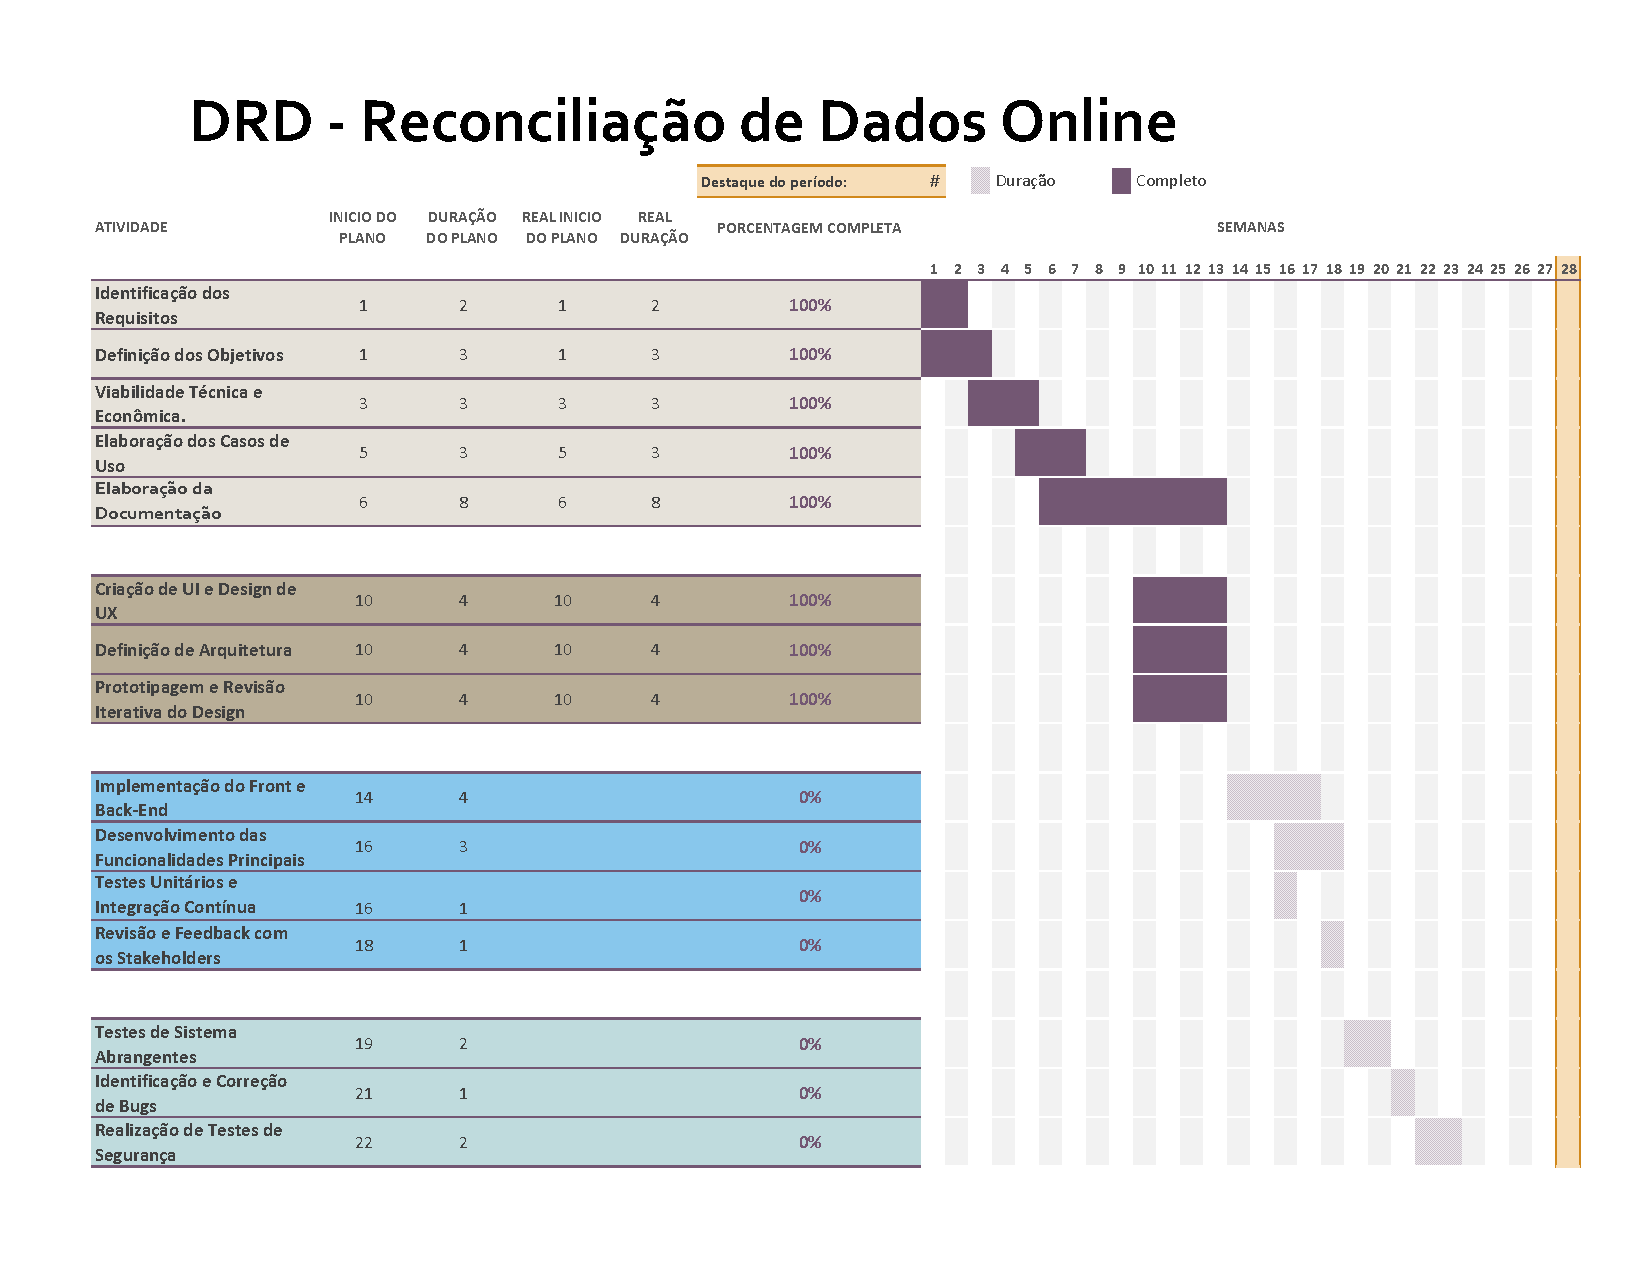
\includegraphics[width=\textwidth]{figuras/DRD-Ganttt.pdf} % Replace "example.pdf" with the path to your PDF file
    \caption{Grafico de Gantt para desenvolvimento do \textit{software} DRD.}
    \label{fig:ganttChart}
\end{figure}    

Na Figura \ref{fig:ganttChart} é visível Gráfico de Gantt utilizado pelo projeto, onde ele é separado nas seguintes partes: 
    
\begin{itemize}
    \item \textbf{Planejamento e Análise Inicial:} Esta fase inclui a identificação dos requisitos, definição dos objetivos, análise de viabilidade técnica e econômica, além da elaboração dos casos de uso e da documentação.
    
    \item \textbf{\textit{Design} e Prototipagem:} Nesta etapa, são criados o design de interface do usuário (UI) e o design de experiência do usuário (UX), bem como a definição da arquitetura do sistema e a prototipagem com revisões iterativas do design.
    
    \item \textbf{Desenvolvimento e Implementação:} Aqui ocorre a implementação do \textit{front} e \textit{back-end}, o desenvolvimento das funcionalidades principais do sistema, os testes unitários e a integração contínua, além da revisão e \textit{feedback} com os \textit{stakeholders}.
    
    \item \textbf{Testes e Garantia de Qualidade:} Esta fase abrange os testes de sistema abrangentes, a identificação e correção de \textit{bugs}, e a realização de testes de segurança para garantir a qualidade do sistema.
    
    \item \textbf{Preparação para Lançamento:} Envolve a preparação do ambiente de produção, o treinamento de usuários finais e o lançamento suave do sistema para garantir uma transição tranquila para os usuários.
    
    \item \textbf{Suporte e Manutenção Pós-Lançamento:} Por fim, inclui o monitoramento contínuo do sistema, atualizações regulares de \textit{software} e fornecimento de suporte técnico aos usuários para garantir o bom funcionamento e a satisfação contínua dos clientes.
\end{itemize}

Desta forma, a utilização do gráfico de Gantt foi crucial, por manter uma organização temporal da produção em razão do tempo decorrido, na qual auxiliou no planejamento e coordenação das diferentes etapas do projeto, permitindo também uma rápida avaliação do progresso do projeto, destacando visualmente as atividades concluídas, as em andamento e as pendentes. Auxiliando a identificar áreas de atraso ou potenciais gargalos, permitindo que a tomada de atitudes corretivas para manter o projeto no caminho certo.
        
\section{Projeto de \textit{Software}}

Descreva o processo de \textit{design} do \textit{software}, incluindo a arquitetura geral do sistema, diagramas de classe, diagramas de sequência, entre outros artefatos de \textit{design}. Explica as decisões de \textit{design} tomadas e como elas estão alinhadas com os requisitos do sistema \cite{softwareeng}.

\subsection{Arquitetura Geral do Sistema}

Durante o desenvolvimento de um \textit{software}, é crucial o uso de representações visuais para uma compreensão mais clara das funcionalidades e estrutura do projeto. Assim, a linguagem de modelagem unificada (UML) permite a criação de diversos tipos de diagramas para representar diferentes aspectos do sistema. Para a solução deste programa, optou-se pelo uso do PlantUML \cite{plantumldoc}, que possibilita a modelagem dos processos através de código, facilitando a alteração e atualização dos diagramas \cite{softwareengreq}.

\subsubsection{Diagrama de Classe}

O diagrama de classes é uma representação visual do projeto na engenharia de \textit{software}, empregada para descrever a estrutura estática de um sistema baseado em objetos \cite{softwareenguml}. Na sua forma mais básica, um diagrama de classes consiste em classes, que são os blocos de construção de um sistema orientado a objetos, contendo os atributos que as características ou propriedades dos objetos dessa classe, enquanto os métodos indicam as operações que podem ser realizadas por esses objetos, como é o caso do diagrama da Figura \ref{fig:ClassDiagram}. Essa estrutura fornece uma representação abstrata e organizada das entidades do sistema, permitindo uma compreensão clara de sua composição e funcionalidades.
            
\begin{figure}[htb]
    \caption{\label{fig:ClassDiagram}Diagrama de Classe em UML.}
    \begin{center}
        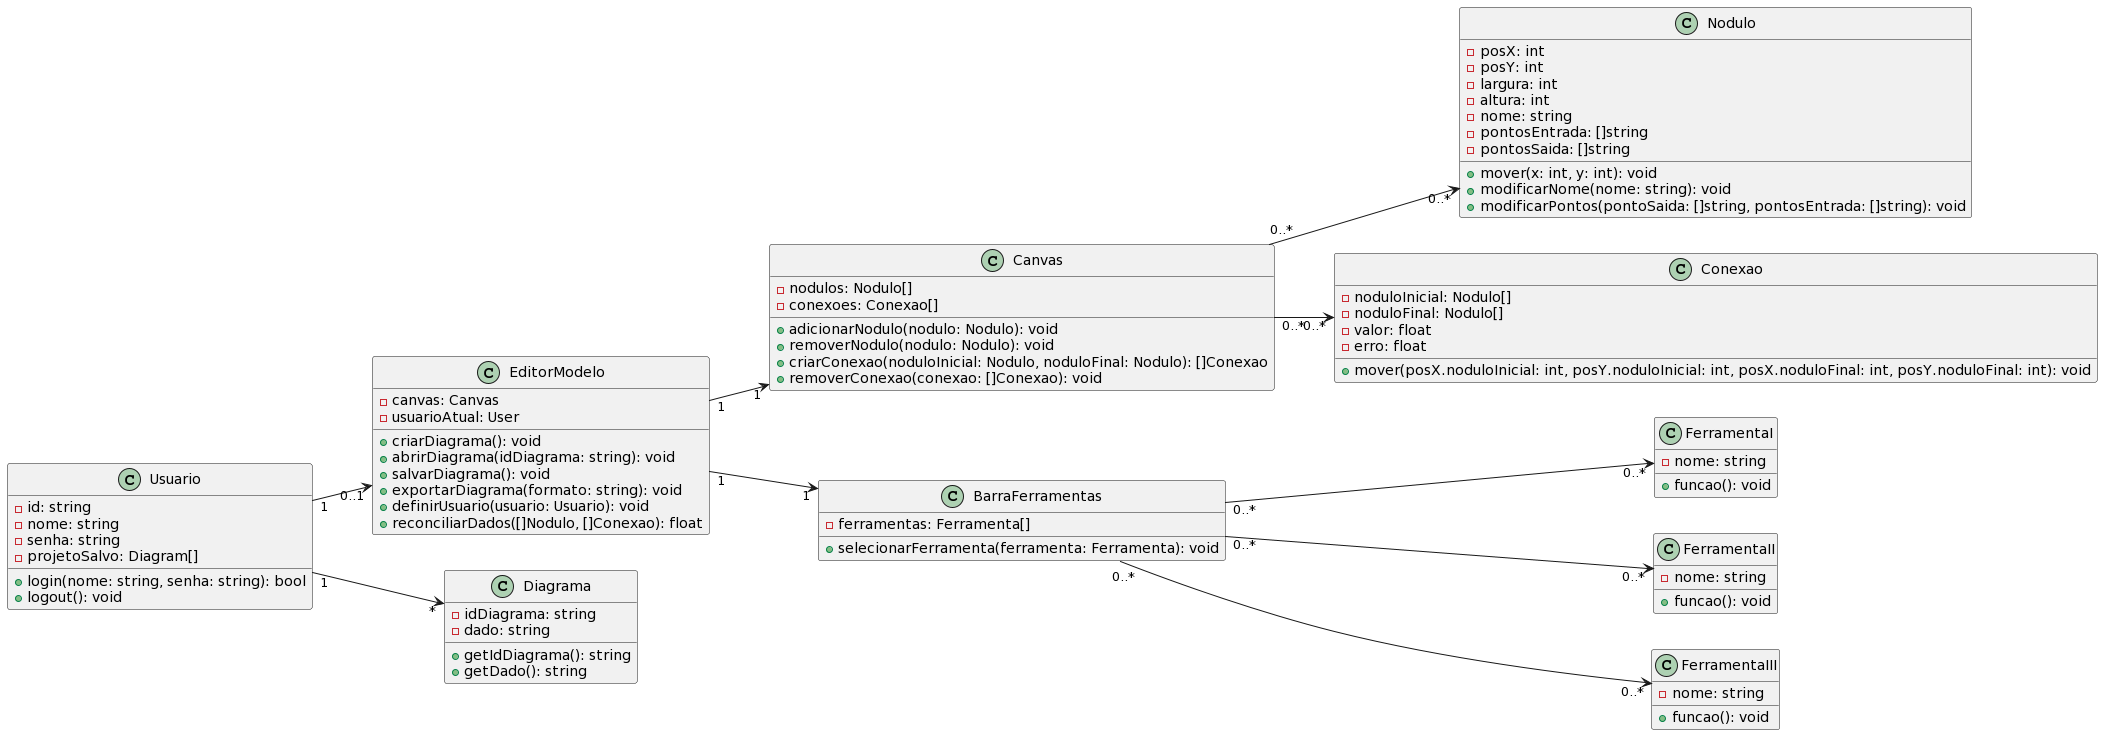
\includegraphics[width=\textwidth]{figuras/ClassDiagram.png}
    \end{center}
\end{figure}
            
Adicionalmente, os relacionamentos entre as classes são destacados por meio de linhas que conectam os blocos das classes. Essas associações podem assumir diferentes formas, como associações simples, agregações, composições, heranças, entre outras, e fornecem \textit{insights} valiosos sobre como as diferentes partes do sistema interagem e dependem umas das outras.
            
Assim, um diagrama de classes torna-se uma ferramenta essencial para modelar a estrutura estática de um sistema, oferecendo uma representação visual nítida das classes, atributos, métodos e seus inter-relacionamentos, o que simplifica o processo de \textit{design}, análise e comunicação entre os integrantes da equipe de desenvolvimento de \textit{software} \cite{softwareenguml}.
            
\subsubsection{Diagrama de Caso de Uso}
        
O diagrama de caso de uso é uma representação visual amplamente utilizada na engenharia de \textit{software} para descrever a interação entre um sistema e seus usuários. Ele destaca os diferentes casos de uso, que representam as diferentes maneiras pelas quais os usuários interagem com o sistema para atingir seus objetivos. Na sua forma mais básica, um diagrama de caso de uso consiste em atores, que são os usuários externos ao sistema, e de casos de uso, que são as diferentes funcionalidades ou serviços oferecidos pelo sistema, como exemplificado no diagrama da Figura \ref{fig:UseCaseDiagram}.
        
\begin{figure}[htb]
    \caption{\label{fig:UseCaseDiagram}Diagrama de Caso de Uso em UML.}
    \begin{center}
        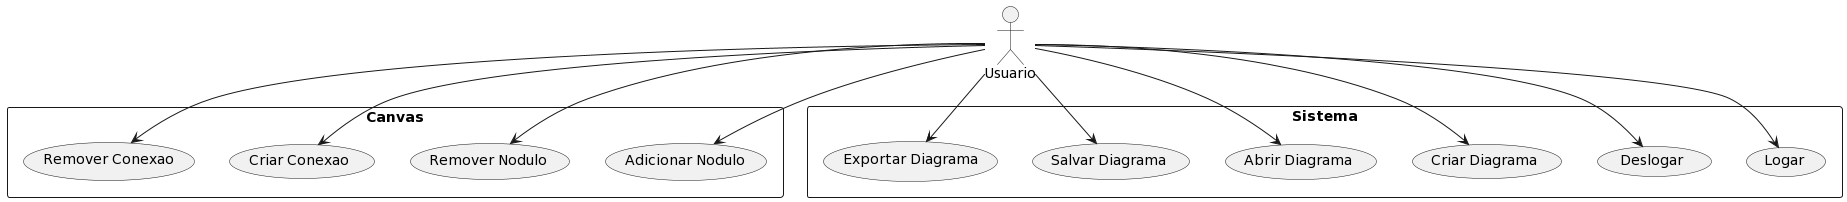
\includegraphics[width=\textwidth]{figuras/UseCaseDiagram.png}
    \end{center}
\end{figure}
        
Os atores representam os diferentes tipos de usuários que interagem com o sistema, enquanto os casos de uso representam as diferentes funcionalidades oferecidas pelo sistema. Esses casos de uso são conectados aos atores por meio de linhas, indicando a interação entre os usuários e as funcionalidades do sistema.
        
Assim, um diagrama de caso de uso torna-se uma ferramenta essencial para modelar a interação entre um sistema e seus usuários, oferecendo uma representação visual clara dos atores, casos de uso e seus inter-relacionamentos. Isso simplifica o processo de \textit{design}, análise e comunicação entre os membros da equipe de desenvolvimento de \textit{software}, garantindo uma implementação eficaz e orientada às necessidades dos usuários.
        
\subsubsection{Diagrama do Banco de Dados}

O diagrama de banco de dados é uma representação visual das estruturas de dados e dos relacionamentos entre elas em um sistema de banco de dados \cite{databasedepth}, na qual visa representar a estrutura dos dados armazenados em um banco de dados e como esses dados estão relacionados entre si, como é o caso da Figura \ref{fig:DatabaseDiagram}, que representa o banco de dados do sistema.
            
\begin{figure}[htb]
    \caption{\label{fig:DatabaseDiagram}Diagrama de Banco de Dados em UML.}
    \begin{center}
        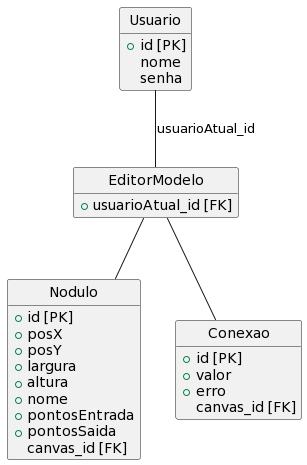
\includegraphics[height=0.25\textheight]{figuras/DatabaseDiagram.png}
    \end{center}
\end{figure}
            
No diagrama de banco de dados, as entidades são representadas por tabelas, onde cada tabela possui colunas que representam os atributos dos dados armazenados. Além disso, as relações entre as tabelas são representadas por meio de chaves estrangeiras, indicando como os dados de uma tabela estão relacionados aos dados de outra tabela.
            
Desta forma, um diagrama de banco de dados é uma ferramenta vital para modelar a estrutura dos dados em um sistema de banco de dados, oferecendo uma representação visual clara das tabelas, colunas e relacionamentos entre elas. Isso facilita o projeto, análise e comunicação entre os membros da equipe de desenvolvimento de \textit{software}, garantindo uma implementação eficiente e eficaz do sistema de banco de dados.
    
\section{Implementação}

O projeto utilizou-se da ferramenta Node.js para gerenciamento de pacotes, permitindo uma gestão eficiente das dependências do projeto. Também foram empregados diversos \textit{plugins} e bibliotecas complementares para facilitar o desenvolvimento e melhorar a experiência do usuário.

O \textit{front-end} do projeto foi implementado utilizando React.js como a principal biblioteca de desenvolvimento de interfaces de usuário. Para estilização, foram empregados arquivos CSS com metodologia BEM (Block Element Modifier) para garantir uma estrutura de estilo escalável e modular. Além disso, o projeto se beneficiou do uso de diversos componentes reutilizáveis para manter um código limpo e organizado \cite{eloquentjavascript}.

Uma outra ferramenta muito utilizada, ainda no \textit{front-end} foi a biblioteca ReactFlow, de criação de diagramas, que foi adaptada para a solução em questão.
    
\section{Gerenciamento de Configuração e Mudança}

Durante o ciclo de vida do desenvolvimento de \textit{software}, foram adotadas diversas práticas e ferramentas para garantir um controle efetivo de versão e gerenciamento de mudanças \cite{gitevery}.
    
Para controle de versão, o Git foi escolhido como sistema de controle de versão distribuído. A plataforma Github \cite{github} foi utilizada para armazenar os repositórios do código-fonte do \textit{software}, o código LaTeX da Trabalho de Conclusão de Curso e da Apresentação. Isso permitiu que a existência de um histórico detalhado de todas as alterações realizadas no código.
    
Além disso, foram estabelecidas políticas de \textit{branches} no Git, como o uso de \textit{branches} de \textit{feature}, \textit{develop} e \textit{main}, para organizar o fluxo de trabalho e facilitar a integração contínua. As alterações no código eram revisadas antes de serem mescladas nos \textit{branches} principais, garantindo a qualidade e consistência do código.
    
Para o gerenciamento de mudanças, uma abordagem baseada em metodologias ágeis foi adotada, utilizando o Scrum. Isso permitiu que as mudanças fossem gerenciadas de forma iterativa e incremental, com entregas frequentes e \textit{feedback} contínuo ao orientador do trabalho.
    
Além disso, foi se utilizado o Trello como ferramenta de rastreamento de problemas \textit{(issue tracking)}, para registrar e acompanhar as mudanças, correções de \textit{bugs} e novas funcionalidades ao longo do desenvolvimento. Isso proporcionou uma visão clara do progresso do projeto e facilitou a comunicação dentro da equipe.
    
Desta forma, o controle de versão e gerenciamento de mudanças foram fundamentais para garantir a integridade, rastreabilidade e qualidade do \textit{software} ao longo de seu desenvolvimento, permitindo uma um comportamento eficaz da e uma entrega de progresso contínua no desenvolvimento do \textit{software}.
% %%
% %% Capítulo 4: Problema
% %%

% \mychapter{Problema2312231}
% \label{Cap:Problema}

% Aqui você deve especificar o seu problema (de forma muito formal). Coloque a matemática (ou descreva a problemática) do problema. Use e abuse de Definições, Teoremas, Proposições e Provas. Descreva a sua solução (matemática) para o problema em questão, como você resolve o problema.
% Pode ser descritivo, mas provando que funciona matematicamente (ou formalmente).

% \section{Elementos flutuantes}
% \label{Sec:flutuantes}

% Uma das maiores dificuldades na edição de textos de qualidade é o
% posicionamento dos elementos gráficos: figuras, gráficos e
% tabelas. Como estes elementos muitas vezes são grandes, aparece o
% dilema sobre o que fazer quando uma quebra de página deveria acontecer
% no meio do elemento. Há duas possibilidades:
% \begin{enumerate}
% \item O autor informa exatamente onde o elemento gráfico deve ficar no
% texto, evitando que quebras de páginas aconteçam no meio de um
% elemento. O problema com esta abordagem é que todo o trabalho de
% posicionamento pode ser perdido caso se inclua ou se exclua algum
% texto ou elemento.
% \item O editor de texto posiciona os elementos gráficos de forma a não
% deixar espaços em branco nas páginas. Estes elementos que podem ser
% posicionados pelo editor são conhecidos como \emph{elementos
% flutuantes}. O problema com esta abordagem é que o posicionamento
% adotado pode não corresponder às expectativas do autor.
% \end{enumerate}

% O \LaTeX\ oferece as duas possibilidades de posicionamento. Este
% capítulo apresenta exemplos de inclusão de elementos gráficos no
% texto, bem como algumas ferramentas externas ao \LaTeX\ que podem ser
% utilizadas para gerá-los.

% Para caracterizar uma parte do texto como sendo flutuante, ela deve ser
% delimitada por \verb|\begin{figure}| e \verb|\end{figure}| ou por
% \verb|\begin{table}| e \verb|\end{table}|. Apesar do que os nomes
% sugerem, nada obriga que o ambiente \texttt{figure} seja usado para
% delimitar figuras ou que o ambiente \texttt{table} seja usado para
% delimitar tabelas, embora esta seja a escolha quase sempre
% adotada. Estes dois ambientes são praticamente equivalentes, com as
% seguintes diferenças:
% \begin{itemize}
% \item os dois ambientes usam contadores diferentes para numerar os
% elementos flutuantes;
% \item os ambientes \texttt{figure} serão incluídos na
% \texttt{listoffigures}, enquanto os ambientes \texttt{table} serão
% incluídos na \texttt{listoftables};
% \item as legendas (\texttt{caption}'s) dos ambientes \texttt{figure}
% serão precedidas da palavra ``Figura \dots'', enquanto as legendas dos
% ambientes \texttt{table} serão precedidas da palavra ``Tabela \dots''.
% Estas duas palavras podem ser alteradas pelo autor.
% \end{itemize}
% Para ilustrar o fato de que estes ambientes podem conter virtualmente
% qualquer coisa, a figura~\ref{Fig:textoflutuante} contém um texto que
% foi tornado flutuante por ser incluído em um ambiente \texttt{figure}
% e as tabelas \ref{Tab:equacaoflutuante} e \ref{Tab:equacaoflutuante2}
% contêm expressões matemáticas flutuantes, incluídas em um ambiente
% \texttt{table}. A tabela (\texttt{table}) \ref{Tab:submultilinhas} na
% página \pageref{Tab:submultilinhas} também não contém uma tabela no
% sentido estrito do termo, mas sim uma linha de texto formada por duas
% \texttt{minipage}'s separadas por um espaço horizontal. A primeira
% \texttt{minipage} contém um trecho de código fonte e a segunda, o
% resultado produzido (uma expressão matemática multialinhada).

% \begin{figure}[tbp]
% \caption{Trecho de \emph{Os Lusíadas}, de Luis de Camões}
% \label{Fig:textoflutuante}
% % hrule - linha horizontal
% \hrule
% % As minipage's são muito úteis para se colocar duas coisas na mesma linha
% \begin{minipage}{0.45\linewidth}
% % flushleft - alinha à esquerda
% \begin{flushleft}
% As armas e os barões assinalados\\
% Que da ocidental praia lusitana\\
% Por mares nunca dantes navegados\\
% Passaram ainda além da Trapobana\\
% Em perigos e guerras esforçados\\
% Mais do que prometia a força humana\\
% Entre gente remota edificaram\\
% Novo reino, que tanto sublimaram
% \end{flushleft}
% \end{minipage}
% \hfill
% \begin{minipage}{0.45\linewidth}
% % flushright - alinha à direita
% \begin{flushright}
% E também as memórias gloriosas\\
% Daqueles reis que foram dilatando\\
% A Fé, o Império, as terras viciosas\\
% De África e Ásia andaram devastando,\\
% E aqueles que por obras valerosas\\
% Se vão da lei da morte libertando:\\
% Cantando espalharei por toda parte,\\
% Se a tanto me ajudar o engenho e arte.
% \end{flushright}
% \end{minipage}
% \hrule
% \end{figure}

% \begin{table}[bp]
% % As minipage's são muito úteis para se colocar duas coisas na mesma linha
% \begin{minipage}[b]{0.45\linewidth}
% \begin{center}
% \[
% ax^2 + bx + c = 0
% \]
% \end{center}
% \caption{Equação de segundo grau}
% \label{Tab:equacaoflutuante}
% \end{minipage}
% \hfill
% \begin{minipage}[b]{0.50\linewidth}
% \begin{center}
% \[
% x = \frac{-b\pm\sqrt{b^2-4ac}}{2a}
% \]
% \end{center}
% \caption{Raízes da equação da tabela~\ref{Tab:equacaoflutuante}}
% \label{Tab:equacaoflutuante2}
% \end{minipage}
% \end{table}

% É importante ressaltar que o que é numerado é o \texttt{caption} e não
% a \texttt{figure} ou a \texttt{table}. Portanto, o \texttt{label} deve
% ser colocado sempre após o \texttt{caption} ao qual ele se
% refere. Conforme ilustram as tabelas \ref{Tab:equacaoflutuante} e
% \ref{Tab:equacaoflutuante2}, uma mesma \texttt{figure} ou
% \texttt{table} pode ter mais de um ou nenhum \texttt{caption}.
% O \texttt{caption} pode ser colocado antes do conteúdo flutuante, como
% na figura \ref{Fig:textoflutuante}, ou depois, como nas tabelas
% \ref{Tab:equacaoflutuante} e \ref{Tab:equacaoflutuante2}. Nos
% documentos do PPgEEC, o padrão é sempre posicionar o \texttt{caption}
% abaixo das figuras e das tabelas.

% \subsection{Posicionamento dos elementos flutuantes}
% \label{Sec:posicionamento}

% Em cada \verb|\begin{figure}| ou \verb|\begin{table}| pode-se incluir
% um parâmetro opcional com as opções de posicionamento para este
% elemento flutuante. Parâmetros adicionais de comandos \LaTeX\ são
% sempre fornecidos entre colchetes \texttt{[]}, enquanto os parâmetros
% obrigatórios aparecem entre chaves \verb|{}|. As opções disponíveis
% incluem as seguintes:
% \begin{itemize}
% \item[\tt h] O elemento pode ser posicionado na mesma posição em que ele
% aparece no código fonte do texto.
% \item[\tt t] O elemento pode ser posicionado no topo de uma página.
% \item[\tt b] O elemento pode ser posicionado no fim de uma página.
% \item[\tt p] O elemento pode ser incluído em uma página formada só por
% flutuantes.
% \item[\tt !] Normalmente o \LaTeX\ faz algumas considerações de ordem
% estética no posicionamento dos flutuantes, o que às vezes faz com que
% alguns elementos sejam posicionados muito longe de onde são citados,
% principalmente se você não incluir a opção \texttt{p}. Para fazer com
% que as considerações estéticas não sejam levadas em conta para um dado
% elemento, inclua a opção \texttt{!}.
% \end{itemize}

% \section{Tabelas em \LaTeX}
% \label{Sec:tabelas}

% Tabelas são construídas com comandos próprios do \LaTeX, notadamente o
% ambiente \texttt{tabular}. Nada obriga a que o ambiente
% \texttt{tabular} esteja sempre posicionado em um elemento
% flutuante. Se você quiser impor que uma tabela fique obrigatoriamente
% em uma determinada posição do texto, basta não colocar o
% \texttt{tabular} dentro de um \texttt{table}. Tabelas podem até ser
% incluídas no meio de uma frase.  Por exemplo, eu posso dizer que se um
% jogo da velha está na configuração \textsf{\tiny\begin{tabular}{c|c|c}
% x & & x \\ \hline & & o \\ \hline x & o & \end{tabular}} e se o
% jogador ``\textsf{x}'' sabe jogar, então o jogador ``\textsf{o}'' irá
% perder, independentemente da jogada que faça.

% O ambiente \texttt{tabular} tem um parâmetro obrigatório que indica o
% número de colunas da tabela e o posicionamento dos objetos em cada
% coluna. Por exemplo, uma tabela criada com \verb|\begin{tabular}{lcr}|
% terá três colunas; o texto será alinhado à esquerda na primeira
% coluna, centralizado na segunda e alinhado à direita na
% terceira. Podem ser incluídos objetos que ocupam mais de uma linha
% (comando \texttt{multirow}) ou mais de uma coluna (comando
% \texttt{multicolumn}). Neste último caso, também é possível mudar o
% alinhamento do texto. Exemplos podem ser vistos nas tabelas
% \ref{Tab:multilinhas} e \ref{Tab:submultilinhas}, na
% página~\pageref{Tab:multilinhas}.

% Com o pacote \texttt{tabularx}, além das opções normais de
% posicionamento de colunas (\texttt{lcr}), pode-se incluir
% automaticamente um texto qualquer antes de cada elemento da coluna
% (\verb|>{}|). Este recurso foi utilizado nas tabelas
% \ref{Tab:multilinhas} e \ref{Tab:submultilinhas} para fazer
% com que todos os textos de algumas colunas fossem automaticamente
% escritos na fonte \texttt{tt}. Além disso, podem-se criar colunas de
% largura fixa e/ou de largura que se ajustam para que a tabela ocupe
% toda a largura desejada, além do estilo tradicional de coluna que
% assume a largura suficiente para conter seus elementos. Exemplos de
% colunas com diferentes larguras e alinhamentos podem ser vistos na
% tabela \ref{Tab:larguracolunas}.

% \begin{table}[htbp]
% \begin{tabularx}{\linewidth}{|p{3cm}|X|l|} \hline
% COLUNA p & COLUNA X & COLUNA l \\ \hline
% Largura fixa (não depende do conteúdo) &
% Expandível &
% Ajustável \\ \hline
% Alinhada no topo &
% Alinhada à esquerda &
% Alinhada à esquerda \\ \hline
% \end{tabularx}
% \\[0.5cm]
% \begin{tabularx}{\linewidth}{|b{3cm}|C|r|} \hline
% COLUNA b & COLUNA C (ver \texttt{comandos.tex}) & COLUNA r \\ \hline
% Largura fixa (não depende do conteúdo) &
% Expandível &
% Ajustável \\ \hline
% Alinhada na base &
% Centralizada &
% Alinhada à direita \\ \hline
% \end{tabularx}
% \caption{Tabelas com colunas de diferentes larguras e alinhamentos}
% \label{Tab:larguracolunas}
% \end{table}

% \section{Figuras em \LaTeX}
% \label{Sec:figuras}

% As figuras (imagens, desenhos, gráficos, etc.) devem ser produzidas
% por ferramentas externas ao \LaTeX, salvas em um arquivo e inseridas
% no texto usando o comando \texttt{includegraphics}. Da mesma forma
% que as tabelas, as figuras podem ser flutuantes, caso sejam
% inseridas dentro de um ambiente \texttt{figure}, ou ter uma posição
% fixa no texto (como aqui: 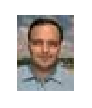
\includegraphics{textuais/04-problema/figuras/eu.eps}).

% O formato em que você deve salvar os arquivos das figuras para que
% possa incluí-las no texto depende de como você pretende compilar
% o código fonte:
% \begin{itemize}
% \item se o texto vai ser compilado com \texttt{latex}, todos os
% arquivos devem estar no formato EPS (\emph{Encapsulated PostScipt});
% \item se o texto vai ser compilado com \texttt{pdflatex}, os
% arquivos devem estar nos formatos PDF ou JPEG (outros formatos são
% aceitos, mas estes são os recomendáveis).
% \end{itemize}
% É aconselhável que você não inclua a terminação no nome do arquivo que
% é parâmetro para o comando \texttt{includegraphics}. Isto porque, de
% acordo com a forma como o texto está sendo compilado, o \LaTeX\
% acrescenta a terminação adequada. Por exemplo, caso seu texto inclua o
% comando \verb|\includegraphics{eu}|, o \LaTeX\ procurará o arquivo
% \texttt{eu.eps} caso esteja sendo chamado via \texttt{latex} ou um dos
% arquivos \texttt{eu.pdf} ou \texttt{eu.jpg} caso esteja sendo chamado
% via \texttt{pdflatex}.

% As figuras podem ser divididas em dois grandes grupos:
% \begin{itemize}
% \item As imagens e fotos, que normalmente correspondem a visões reais
% do mundo e são obtidas por câmeras digitais ou
% assemelhados. Caracterizam-se por conterem grandes quantidades de
% nuances, texturas e cores.
% \item As figuras sintéticas, normalmente produzidas utilizando
% \emph{softwares} dedicados. Geralmente contêm figuras geométricas
% (linhas, quadrados, etc.), textos e poucas cores e texturas. Neste
% grupo, para efeito de discussão das ferramentas de produção, podem-se
% identificar duas categorias:
% \begin{itemize}
% \item Os desenhos e esquemas: diagramas de blocos, organogramas e
% fluxogramas, representações esquemáticas, etc.
% \item Os gráficos: representações gráficas de valores ou funções
% matemáticas.
% \end{itemize}
% \end{itemize}

% \subsection{Imagens e fotos}
% \label{Sec:imagens}

% As imagens e fotos normalmente só podem ser armazenadas em formatos
% que representam cada \emph{pixel} da imagem separadamente,
% eventualmente com algum tipo de compressão. Os formatos JPEG, GIF,
% TIF, PNM (PBM, PGM ou PPM), BMP (Bitmap) e PNG, entre outros, são
% todos desta categoria.  Se sua figura está em algum destes formatos,
% você deve convertê-la para EPS (se usar \texttt{latex}) ou para JPEG
% (se usar \texttt{pdflatex}) para poder incluí-la no documento \LaTeX.

% A quase totalidade dos \emph{softwares} de visualização de imagens
% permite salvá-las em múltiplos formatos, geralmente incluindo JPEG e
% EPS. No Unix, você dispõe ainda de vários programas para fazer a
% conversão em comandos de linha: \texttt{jpegtopnm},
% \texttt{pnmtojpeg}, \texttt{pnmtops}, \texttt{gif2ps},
% \texttt{giftopnm}, \texttt{tiff2ps}, \texttt{tifftopnm},
% \texttt{bmptopnm} e \texttt{pngtopnm}, entre outros.

% A figura \ref{Fig:belmonte} mostra um exemplo de inclusão de uma
% imagem no texto \LaTeX.

% \begin{figure}[htbp!] \begin{center}
% % fbox faz uma borda ao redor do seu argumento
% \fbox{\includegraphics[width=0.75\linewidth]{textuais/04-problema/figuras/belmonte}}
% \caption{Exemplo de imagem real}
% \label{Fig:belmonte}
% \end{center} \end{figure}

% \subsection{Figuras sintéticas}
% \label{Sec:figsinteticas}

% As figuras sintéticas podem ser armazenadas em formato
% \emph{pixel}-a-\emph{pixel}, como se fossem uma imagem, ou em
% formato vetorial. No formato vetorial as primitivas que formam a
% figura (linhas, textos, etc.) são descritas pelos parâmetros que as
% caracterizam (ponto de início e fim, \emph{string} e posição do texto,
% etc.). As figuras em formato vetorial são mais adequadas pois
% usualmente correspondem a arquivos menores e a qualidade da imagem
% não sofre perdas ao se aumentar ou diminuir o tamanho da figura.

% Para inclusão no \LaTeX, os formatos PDF e EPS são os únicos que podem
% representar figuras no formato vetorial. Nem toda figura salva nestes
% formatos, entretanto, é necessariamente vetorial, pois tanto o PDF
% quanto o EPS podem representar tanto figuras em formato
% \emph{pixel}-a-\emph{pixel} quanto figuras em formato vetorial. Para
% que sua figura seja vetorial, é necessário que o \emph{software} que a
% gerou tenha a capacidade de produzi-las.

% Para demonstrar a melhor qualidade das figuras em formato vetorial,
% nas figuras \ref{Fig:bigvetorial} e \ref{Fig:bigbitmap} se mostra em
% tamanho natural um mesmo diagrama nos formatos vetorial e de
% \emph{pixels}. Nas figuras \ref{Fig:bigvetorialreduzida} e
% \ref{Fig:bigbitmapreduzida} estas mesmas figuras são apresentadas
% com uma redução de 50\%, utilizando o parâmetro \texttt{scale} do
% \texttt{includegraphics}. Já nas figuras \ref{Fig:smallvetorial} e
% \ref{Fig:smallbitmap} o diagrama original foi reduzido, de forma que
% seu tamanho natural é menor. Nas figuras
% \ref{Fig:smallvetorialampliada} e \ref{Fig:smallbitmapampliada}
% este diagrama pequeno está aumentado de um fator arbitrário, calculado
% pelo \texttt{includegraphics} para que a imagem ocupe toda a largura
% da linha.

% \begin{figure}[htbp!] 
%     \begin{center}
%         \includegraphics{textuais/04-problema/figuras/bigvetorial}
%         \caption{Figura vetorial grande em tamanho natural}
%         \vspace{6mm}
%         \label{Fig:bigvetorial}
%     \end{center} 
% \end{figure}

% \begin{figure}[htbp!] \begin{center}
% \includegraphics{textuais/04-problema/figuras/smallvetorial}
% \caption{Figura vetorial pequena em tamanho natural}
% \label{Fig:smallvetorial}
% \vspace{6mm}
% \includegraphics{textuais/04-problema/figuras/smallbitmap}
% \caption{Figura \emph{pixel}-a-\emph{pixel} pequena em tamanho natural}
% \label{Fig:smallbitmap}
% \vspace{6mm}
% \includegraphics[width=\linewidth]{textuais/04-problema/figuras/smallvetorial}
% \caption{Figura vetorial pequena em tamanho ampliado}
% \label{Fig:smallvetorialampliada}
% \vspace{6mm}
% \includegraphics[width=\linewidth]{textuais/04-problema/figuras/smallbitmap}
% \caption{Figura \emph{pixel}-a-\emph{pixel} pequena em tamanho ampliado}
% \label{Fig:smallbitmapampliada}
% \end{center} \end{figure}

% Nota-se que no formato vetorial as
% linhas mantêm a espessura mesmo quando se fazem
% ampliações ou reduções. Já no formato de \emph{pixels}
% as linhas ficam mais claras (cinzas, ao invés de pretas) após as
% reduções e mais grossas após as ampliações, além de uma perda geral
% de definição da imagem.

% \section{Ferramentas para desenhos e esquemas}
% \label{Sec:desenhos}

% Existem diversas ferramentas para fazer desenhos, mas muitas delas
% apenas salvam a figura gerada em formatos \emph{pixel}-a-\emph{pixel}.
% No Unix, pode-se utilizar o \texttt{xfig}, que exporta imagens em
% muitos formatos, inclusive nos vetoriais (PDF e EPS). Os diagramas das
% figuras \ref{Fig:bigvetorial} a \ref{Fig:smallbitmapampliada} foram
% desenhados e exportados no \texttt{xfig}. O arquivo fonte
% correspondente é o \texttt{diagrama.fig}, no diretório
% \texttt{figuras}.

% A possibilidade de salvar figuras em modo vetorial impõe que alguns
% recursos para desenho de imagens não sejam oferecidos. Um deles é o
% desenho a mão-livre, já que seria impossível descrever a curva obtida
% em termos de figuras geométricas básicas. Outro recurso inexistente é
% o de preencher uma região com uma determinada cor. Esta última
% limitação muitas vezes pode ser contornada utilizando-se a noção de
% profundidade.  Por exemplo, para desenhar uma figura vazado e
% preenchido de azul, pode-se desenhar a figura externa preenchido de
% azul sobre o qual se desenha a figura interna preenchido de branco,
% como mostram os exemplos da figura~\ref{Fig:circulo}.

% \begin{figure}[htb] \begin{center}
% \includegraphics{textuais/04-problema/figuras/circulo}
% \caption{Preenchimento de figuras utilizando diferentes profundidades}
% \label{Fig:circulo}
% \end{center} \end{figure}

% %A noção de profundidade no \texttt{xfig} foi exaustivamente utilizada
% %para desenhar os símbolos da UFRN e do PPgEEC que podem ser vistos na
% %página de rosto deste documento. 
% %Os arquivos \texttt{xfig} correspondentes são \texttt{UFRN.fig} e \texttt{PPgEE.fig}. 
% A noção de profundidade no \texttt{xfig} pode ser utilizada para mesclar imagens com figuras sintéticas, como na figura \ref{Fig:pensador} (veja arquivo \texttt{figuras/pensador.fig}).

% \begin{figure}[htb] \begin{center}
% \includegraphics{textuais/04-problema/figuras/pensador}
% \caption{Imagem mesclada com elementos sintéticos}
% \label{Fig:pensador}
% \end{center} \end{figure}

% Outra possibilidade oferecida pelo \texttt{xfig} é a inclusão de comandos
% \LaTeX\ dentro da figura. Para utilizar este recurso,
% marque no \texttt{xfig} os textos que devem ser interpretados como
% comandos \LaTeX\ com o \emph{flag} \texttt{special} e exporte a figura
% no modo \emph{Combinado PS/Latex} ou \emph{Combinado PDF/Latex}. Veja
% um exemplo na figura \ref{Fig:combinado}; note que o arquivo é incluído com
% \verb|\input{}| e não com \verb|\includegraphics{}|.

% % Note que foi redefinido um comando aqui no texto para ser incluído
% % na figura. Isto é para evitar digitação de expressões LaTeX muito
% % grandes dentro do xfig
% \newcommand{\formulagrande}{$\frac{G_3G_4}{1-G_3G_4H_1}$}
% \begin{figure}[htb] \begin{center}
% %\input{textuais/04-problema/figuras/combinado.pstex_t} % Se usar latex
% \input{textuais/04-problema/figuras/combinado.pdftex_t} % Se usar pdflatex
% \caption{Figura incluindo comandos \LaTeX}
% \label{Fig:combinado}
% \end{center} \end{figure}

% \section{Ferramentas para gráficos}
% \label{Sec:graficos}

% Gráficos devem ser gerados com aplicativos capazes de exportar o
% resultado nos formatos EPS ou PDF, preferencialmente em formato
% vetorial. Os conhecidos programas \emph{Scilab} e \emph{Matlab} têm
% esta capacidade. Se você deseja algo mais simples, a ferramenta
% \textit{GNUplot} é uma das mais utilizadas no Unix para a geração de
% gráficos de funções matemáticas.

% Uma vez gerados, gráficos são inseridos no texto tal como figuras. A
% figura~\ref{fig:grafico} apresenta um gráfico gerado através do
% comando de linha \texttt{gnuplot grafico.gnuplot}. Este arquivo
% \texttt{grafico.gnuplot}, que contém uma série de comandos do
% \textit{GNUplot}, está no diretório \texttt{figuras}.

% \begin{figure}[htbp]
% \centering
% \includegraphics{textuais/04-problema/figuras/grafico}
% \caption{Exemplo de gráfico de funções matemáticas}
% \label{fig:grafico}
% \end{figure}

% \section{Conclusões}

% Ferramentas de desenho capazes de gerar a saída em formato vetorial
% são mais difíceis de usar e parecem ser dotadas de menos recursos do
% que outras que só exportam seus resultados como imagens de
% \emph{pixels}.  Isto se deve à necessidade de descrever todos os
% elementos da imagem sob a forma de primitivas parametrizáveis para
% permitir que elas sejam escaláveis à vontade e exportáveis para
% qualquer formato desejado.

% Entretanto, a qualidade visual das figuras obtidas e a sua
% reusabilidade é muito maior. A comparação é aproximadamente a mesma
% que a entre textos produzidos em \LaTeX\ e em editores gráficos. Desta
% forma, na medida do possível, tente conjugar a escrita do documento
% \LaTeX\ com a utilização de alguma ferramenta de desenho vetorial.

% % LocalWords:  editadas PS

%%
%% Capítulo 4: Figuras, gráficos e tabelas
%%

\mychapter{Implementação}
\label{Cap:Implementacao}

Coloque aqui a parte sistêmica da solução do problema. Para isto, monte um diagrama de blocos, descrevendo cada caixinha do diagrama. Caso o seu trabalho lide com engenharia de \textit{software}, você também pode apresentar também outros tipos de diagrama (casos de uso, classes, modelos entidade-relacionamento, entre outros), desde que saiba o que eles significam. Diga qual a linguagem, máquina e outras informações técnicas. Coloque os algoritmos ou técnicas implementadas que resolveram o problema especificado formalmente no capítulo anterior. Use e abuse de textos como ``este algoritmo implementa a equação xx do Capítulo YY'', para fazer referência aosCa formalismos definidos nos capítulos \ref{Cap:Metodologia} e \ref{Cap:apendiceA}.

\section{Algoritmos}
\label{Sec:algoritmos}

O latex provê alguns pacotes para a montagem de algoritmos. Um destes pacotes é o \texttt{algorithm2e}, que permite o uso de diretivas de comando em português. De acordo com o manual do pacote, os comandos disponíveis em português são os seguintes:


\begin{itemize}
\item Entradas e saídas do algoritmo:
	\begin{itemize}
 	\item \verb|\Entrada{Entrada}| $\rightarrow$ \textbf{KwEntrada};
 	\item \verb|\Saida{Saída}| $\rightarrow$ \textbf{KwSaida};
 	\item \verb|\Dados{Dados}| $\rightarrow$ \textbf{KwDados};
 	\item \verb|\Resultado{Resultado}| $\rightarrow$ \textbf{KwResultado}.
 	\end{itemize}
\item Retorno do algoritmo:
	\begin{itemize}
 		\item \verb|\Ate| $\rightarrow$ \textbf{at\'{e}};
 		\item \verb|\KwRetorna{[valor]}| $\rightarrow$ \textbf{KwRetorna};
 		\item \verb|\Retorna{[valor]}| $\rightarrow$ \textbf{Retorna}.
 	\end{itemize}
\item Início de bloco: \verb|\Iniciob{bloco interno}| $\rightarrow$ \textbf{Iniciob}.
\item Condicionais (\textit{if-then-else}):
	\begin{itemize} 
		\item \verb|\eSe{condição}{bloco `then'}{bloco `else'}| $\rightarrow$ \textbf{eSe};
 		\item \verb|\Se{condição}{bloco `then'}| $\rightarrow$ \textbf{Se};
 		\item \verb|\uSe{condição}{bloco `else'' sem `fim'}| $\rightarrow$ \textbf{uSe};
 		\item \verb|\lSe{condição}{linha de texto `then'}| $\rightarrow$ \textbf{lSe};
 		\item \verb|\Senao{bloco `else'}| $\rightarrow$ \textbf{Senão};
 		\item \verb|\uSenao{bloco `else' sem `else'}| $\rightarrow$ \textbf{uSenão};
 		\item \verb|\lSenao{linha de código ``else''}| $\rightarrow$ \textbf{lSenão};
 		\item \verb|\SenaoSe{condição}{bloco ``else-if''}| $\rightarrow$ \textbf{uSenãoSe};
		\item \verb|\uSenaoSe{condição}{bloco ``else-if'' sem ``fim''}| $\rightarrow$ \textbf{uSenãoSe};
 		\item \verb|\lSenaoSe{condição}{linha de códigoo ``else-if''}| $\rightarrow$ \textbf{lSenãoSe}.
 	\end{itemize}
\item Seleção de casos (\textit{switch-case}):
	\begin{itemize}
		\item \verb|\Selec{condição}{bloco `switch'}| $\rightarrow$ \textbf{Selec};
  		\item \verb|\Caso{um caso}{bloco `case'}| $\rightarrow$ \textbf{Caso};
  		\item \verb|\uCaso{um caso}{bloco `case' sem `fim'}| $\rightarrow$ \textbf{uCaso};
  		\item \verb|\lCaso{um caso}{linha de código `case'}| $\rightarrow$ \textbf{lCaso};
  		\item \verb|\Outro{bloco `outros'}| $\rightarrow$ \textbf{Outro};
  		\item \verb|\lOutro{linha de código`outros'}| $\rightarrow$ \textbf{lOutro}.
  	\end{itemize}
\item Laços \textit{for}:
	\begin{itemize}
		\item \verb|\Para{condição}{bloco de repetição}| $\rightarrow$ \textbf{Para};
  		\item \verb|\lPara{condição}{linha de código de repetição}| $\rightarrow$ \textbf{lPara};
		\item \verb|\ParaPar{condição}{bloco de repetição}| $\rightarrow$ \textbf{ParaPar};
  		\item \verb|\lParaPar{condição}{linha de código de repetição}| $\rightarrow$ \textbf{lParaPar} ;
  		\item \verb|\ParaCada{condição}{bloco de repetição}| $\rightarrow$ \textbf{ParaCada};
  		\item \verb|\lParaCada{condição}{linha de código de repetição}| $\rightarrow$ \textbf{lParaCada};
		\item \verb|\ParaTodo{condição}{bloco de repetição}| $\rightarrow$ \textbf{ParaTodo};
  		\item \verb|\lParaTodo{condição}{linha de código de repetição}| $\rightarrow$ \textbf{lParaTodo}.
	\end{itemize}
\item Laços \textit{while}:
	\begin{itemize}
		\item \verb|\Enqto{condição de parada}{bloco de repetição}| $\rightarrow$ \textbf{Enqto};
  		\item \verb|\lEnqto{condição de parada}{bloco de repetição}| $\rightarrow$ \textbf{lEnqto}.
	\end{itemize}
\item Laços \textit{do-while}:
	\begin{itemize}
		\item \verb|\Repita{condição de parada}{bloco de repetição}| $\rightarrow$ \textbf{Repita};
  		\item \verb|\lRepita{condição de parada}{linha de código de repetição}| $\rightarrow$ \textbf{lRepita}.
  	\end{itemize}
\item Comentários: \verb|\tcc{comentário}|.
\end{itemize}

Os algoritmos \ref{algo:1} e \ref{algo:2} apresentam alguns modelos de algoritmos para serem tomados de exemplo.

\begin{algorithm}
%% \SetLine
\Entrada{$x$: vetores de valores; $y$ = $L(x)$; $p$: valor de entrada a ser calculado }
\Saida{$s$ = $L(p)$}
$n \leftarrow \mathtt{comprimento}(x)$\;
$s \leftarrow 0$\;
\Para {$i=1$ \Ate $n$} {
	$L \leftarrow 1$\;
	\Para {$j=1:1:n$} {
		\Se{$i \neq j$} {
			$L \leftarrow L* \left( \dfrac{p-x[j]}{x[i]-x[j]} \right) $
		}
	}
	$s \leftarrow s + L*y[i]$\;
}
\Retorna $s$\;
\caption{Algoritmo para interpolação de Lagrange.}
\label{algo:1}
\end{algorithm}

\begin{algorithm}
%% \SetLine
\Entrada{$a$: valor inicial; $b$: valor final; $n$: número de subintervalos (deve ser múltiplo de 2)  }
\tcc{A função a ser integrada é definida em uma função denominada \texttt{f}, fora do escopo deste algoritmo.}
\Saida{$I$ = integral de \texttt{f} entre $a$ e $b$}
$h \leftarrow$ $\dfrac{b-a}{n}$\;
$x[1] \leftarrow a$\;
$y[1] \leftarrow f(a)$\;
$I \leftarrow 0$\;
$k \leftarrow 2$\;
\Enqto {$k <= n$} {
	$x[i] \leftarrow x[i-1] + h$\;
	$y[i] \leftarrow f(x[i])$\;
	\eSe{$i \% 2 = 0$} {
		$I \leftarrow I + 4*y[i]$\;
	}
	{
		$I \leftarrow I + 2*y[i]$\;
	}
	$k = k+1$\;
}
$x[n+1] \leftarrow b$\;
$y[n+1] \leftarrow f(x[i+1])$\;
$I \leftarrow I + \dfrac{h}{3}*(I + y[n+1])$\;
\Retorna $I$\;
\caption{Algoritmo para a integração pelo primeiro método de Simpson.}
\label{algo:2}
\end{algorithm}

%%
%% Capítulo 4: Figuras, gráficos e tabelas
%%

\mychapter{Experimentos e Resultados}
\label{Cap:ExperimentosResultados}

Esta é a parte mais importante (e interessante) do trabalho. Especifique o ferramental usado para a experimentação empírica da solução implementada. Descreva cada experimento realizado de forma bem explicativa (ou seja, planeje os experimentos). Veja o que experimentar, o que são resultados (erros e métricas usadas para medi-los, medidas estatísticas). Use e abuse de gráficos, tabelas e figuras mostrando resultados visuais (impressiona). Uma dica interessante: faça um video e coloque no youtube, demonstrando o sistema funcionando (impressiona), citando a URL entre parênteses. Não apenas descreva os experimentos, mas também discuta os resultados e os compare (principalmente) com outros encontrados na literatura (e citados nos trabalhos relacionados).

%Uma das maiores dificuldades na edição de textos de qualidade é o
%posicionamento dos elementos gráficos: figuras, gráficos e
%tabelas. Como estes elementos muitas vezes são grandes, aparece o
%dilema sobre o que fazer quando uma quebra de página deveria acontecer
%no meio do elemento. Há duas possibilidades:
%\begin{enumerate}
%\item O autor informa exatamente onde o elemento gráfico deve ficar no
%texto, evitando que quebras de páginas aconteçam no meio de um
%elemento. O problema com esta abordagem é que todo o trabalho de
%posicionamento pode ser perdido caso se inclua ou se exclua algum
%texto ou elemento.
%\item O editor de texto posiciona os elementos gráficos de forma a não
%deixar espaços em branco nas páginas. Estes elementos que podem ser
%posicionados pelo editor são conhecidos como \emph{elementos
%flutuantes}. O problema com esta abordagem é que o posicionamento
%adotado pode não corresponder às expectativas do autor.
%\end{enumerate}
%
%O \LaTeX\ oferece as duas possibilidades de posicionamento. Este
%capítulo apresenta exemplos de inclusão de elementos gráficos no
%texto, bem como algumas ferramentas externas ao \LaTeX\ que podem ser
%utilizadas para gerá-los.
%
%\section{Elementos flutuantes}
%\label{Sec:flutuantes}
%
%Para caracterizar uma parte do texto como sendo flutuante, ela deve ser
%delimitada por \verb|\begin{figure}| e \verb|\end{figure}| ou por
%\verb|\begin{table}| e \verb|\end{table}|. Apesar do que os nomes
%sugerem, nada obriga que o ambiente \texttt{figure} seja usado para
%delimitar figuras ou que o ambiente \texttt{table} seja usado para
%delimitar tabelas, embora esta seja a escolha quase sempre
%adotada. Estes dois ambientes são praticamente equivalentes, com as
%seguintes diferenças:
%\begin{itemize}
%\item os dois ambientes usam contadores diferentes para numerar os
%elementos flutuantes;
%\item os ambientes \texttt{figure} serão incluídos na
%\texttt{listoffigures}, enquanto os ambientes \texttt{table} serão
%incluídos na \texttt{listoftables};
%\item as legendas (\texttt{caption}'s) dos ambientes \texttt{figure}
%serão precedidas da palavra ``Figura \dots'', enquanto as legendas dos
%ambientes \texttt{table} serão precedidas da palavra ``Tabela \dots''.
%Estas duas palavras podem ser alteradas pelo autor.
%\end{itemize}
%Para ilustrar o fato de que estes ambientes podem conter virtualmente
%qualquer coisa, a figura~\ref{Fig:textoflutuante} contém um texto que
%foi tornado flutuante por ser incluído em um ambiente \texttt{figure}
%e as tabelas \ref{Tab:equacaoflutuante} e \ref{Tab:equacaoflutuante2}
%contêm expressões matemáticas flutuantes, incluídas em um ambiente
%\texttt{table}. A tabela (\texttt{table}) \ref{Tab:submultilinhas} na
%página \pageref{Tab:submultilinhas} também não contém uma tabela no
%sentido estrito do termo, mas sim uma linha de texto formada por duas
%\texttt{minipage}'s separadas por um espaço horizontal. A primeira
%\texttt{minipage} contém um trecho de código fonte e a segunda, o
%resultado produzido (uma expressão matemática multialinhada).
%
%\begin{figure}[tbp]
%\caption{Trecho de \emph{Os Lusíadas}, de Luis de Camões}
%\label{Fig:textoflutuante}
%% hrule - linha horizontal
%\hrule
%% As minipage's são muito úteis para se colocar duas coisas na mesma linha
%\begin{minipage}{0.45\linewidth}
%% flushleft - alinha à esquerda
%\begin{flushleft}
%As armas e os barões assinalados\\
%Que da ocidental praia lusitana\\
%Por mares nunca dantes navegados\\
%Passaram ainda além da Trapobana\\
%Em perigos e guerras esforçados\\
%Mais do que prometia a força humana\\
%Entre gente remota edificaram\\
%Novo reino, que tanto sublimaram
%\end{flushleft}
%\end{minipage}
%\hfill
%\begin{minipage}{0.45\linewidth}
%% flushright - alinha à direita
%\begin{flushright}
%E também as memórias gloriosas\\
%Daqueles reis que foram dilatando\\
%A Fé, o Império, as terras viciosas\\
%De África e Ásia andaram devastando,\\
%E aqueles que por obras valerosas\\
%Se vão da lei da morte libertando:\\
%Cantando espalharei por toda parte,\\
%Se a tanto me ajudar o engenho e arte.
%\end{flushright}
%\end{minipage}
%\hrule
%\end{figure}
%
%\begin{table}[bp]
%% As minipage's são muito úteis para se colocar duas coisas na mesma linha
%\begin{minipage}[b]{0.45\linewidth}
%\begin{center}
%\[
%ax^2 + bx + c = 0
%\]
%\end{center}
%\caption{Equação de segundo grau}
%\label{Tab:equacaoflutuante}
%\end{minipage}
%\hfill
%\begin{minipage}[b]{0.50\linewidth}
%\begin{center}
%\[
%x = \frac{-b\pm\sqrt{b^2-4ac}}{2a}
%\]
%\end{center}
%\caption{Raízes da equação da tabela~\ref{Tab:equacaoflutuante}}
%\label{Tab:equacaoflutuante2}
%\end{minipage}
%\end{table}
%
%É importante ressaltar que o que é numerado é o \texttt{caption} e não
%a \texttt{figure} ou a \texttt{table}. Portanto, o \texttt{label} deve
%ser colocado sempre após o \texttt{caption} ao qual ele se
%refere. Conforme ilustram as tabelas \ref{Tab:equacaoflutuante} e
%\ref{Tab:equacaoflutuante2}, uma mesma \texttt{figure} ou
%\texttt{table} pode ter mais de um ou nenhum \texttt{caption}.
%O \texttt{caption} pode ser colocado antes do conteúdo flutuante, como
%na figura \ref{Fig:textoflutuante}, ou depois, como nas tabelas
%\ref{Tab:equacaoflutuante} e \ref{Tab:equacaoflutuante2}. Nos
%documentos do PPgEE, o padrão é sempre posicionar o \texttt{caption}
%abaixo das figuras e das tabelas.
%
%\subsection{Posicionamento dos elementos flutuantes}
%\label{Sec:posicionamento}
%
%Em cada \verb|\begin{figure}| ou \verb|\begin{table}| pode-se incluir
%um parâmetro opcional com as opções de posicionamento para este
%elemento flutuante. Parâmetros adicionais de comandos \LaTeX\ são
%sempre fornecidos entre colchetes \texttt{[]}, enquanto os parâmetros
%obrigatórios aparecem entre chaves \verb|{}|. As opções disponíveis
%incluem as seguintes:
%\begin{itemize}
%\item[\tt h] O elemento pode ser posicionado na mesma posição em que ele
%aparece no código fonte do texto.
%\item[\tt t] O elemento pode ser posicionado no topo de uma página.
%\item[\tt b] O elemento pode ser posicionado no fim de uma página.
%\item[\tt p] O elemento pode ser incluído em uma página formada só por
%flutuantes.
%\item[\tt !] Normalmente o \LaTeX\ faz algumas considerações de ordem
%estética no posicionamento dos flutuantes, o que às vezes faz com que
%alguns elementos sejam posicionados muito longe de onde são citados,
%principalmente se você não incluir a opção \texttt{p}. Para fazer com
%que as considerações estéticas não sejam levadas em conta para um dado
%elemento, inclua a opção \texttt{!}.
%\end{itemize}
%
%\section{Tabelas em \LaTeX}
%\label{Sec:tabelas}
%
%Tabelas são construídas com comandos próprios do \LaTeX, notadamente o
%ambiente \texttt{tabular}. Nada obriga a que o ambiente
%\texttt{tabular} esteja sempre posicionado em um elemento
%flutuante. Se você quiser impor que uma tabela fique obrigatoriamente
%em uma determinada posição do texto, basta não colocar o
%\texttt{tabular} dentro de um \texttt{table}. Tabelas podem até ser
%incluídas no meio de uma frase.  Por exemplo, eu posso dizer que se um
%jogo da velha está na configuração \textsf{\tiny\begin{tabular}{c|c|c}
%x & & x \\ \hline & & o \\ \hline x & o & \end{tabular}} e se o
%jogador ``\textsf{x}'' sabe jogar, então o jogador ``\textsf{o}'' irá
%perder, independentemente da jogada que faça.
%
%O ambiente \texttt{tabular} tem um parâmetro obrigatório que indica o
%número de colunas da tabela e o posicionamento dos objetos em cada
%coluna. Por exemplo, uma tabela criada com \verb|\begin{tabular}{lcr}|
%terá três colunas; o texto será alinhado à esquerda na primeira
%coluna, centralizado na segunda e alinhado à direita na
%terceira. Podem ser incluídos objetos que ocupam mais de uma linha
%(comando \texttt{multirow}) ou mais de uma coluna (comando
%\texttt{multicolumn}). Neste último caso, também é possível mudar o
%alinhamento do texto. Exemplos podem ser vistos nas tabelas
%\ref{Tab:multilinhas} e \ref{Tab:submultilinhas}, na
%página~\pageref{Tab:multilinhas}.
%
%Com o pacote \texttt{tabularx}, além das opções normais de
%posicionamento de colunas (\texttt{lcr}), pode-se incluir
%automaticamente um texto qualquer antes de cada elemento da coluna
%(\verb|>{}|). Este recurso foi utilizado nas tabelas
%\ref{Tab:multilinhas} e \ref{Tab:submultilinhas} para fazer
%com que todos os textos de algumas colunas fossem automaticamente
%escritos na fonte \texttt{tt}. Além disso, podem-se criar colunas de
%largura fixa e/ou de largura que se ajustam para que a tabela ocupe
%toda a largura desejada, além do estilo tradicional de coluna que
%assume a largura suficiente para conter seus elementos. Exemplos de
%colunas com diferentes larguras e alinhamentos podem ser vistos na
%tabela \ref{Tab:larguracolunas}.
%
%\begin{table}[htbp]
%\begin{tabularx}{\linewidth}{|p{3cm}|X|l|} \hline
%COLUNA p & COLUNA X & COLUNA l \\ \hline
%Largura fixa (não depende do conteúdo) &
%Expandível &
%Ajustável \\ \hline
%Alinhada no topo &
%Alinhada à esquerda &
%Alinhada à esquerda \\ \hline
%\end{tabularx}
%\\[0.5cm]
%\begin{tabularx}{\linewidth}{|b{3cm}|C|r|} \hline
%COLUNA b & COLUNA C (ver \texttt{comandos.tex}) & COLUNA r \\ \hline
%Largura fixa (não depende do conteúdo) &
%Expandível &
%Ajustável \\ \hline
%Alinhada na base &
%Centralizada &
%Alinhada à direita \\ \hline
%\end{tabularx}
%\caption{Tabelas com colunas de diferentes larguras e alinhamentos}
%\label{Tab:larguracolunas}
%\end{table}
%
%\section{Figuras em \LaTeX}
%\label{Sec:figuras}
%
%As figuras (imagens, desenhos, gráficos, etc.) devem ser produzidas
%por ferramentas externas ao \LaTeX, salvas em um arquivo e inseridas
%no texto usando o comando \texttt{includegraphics}. Da mesma forma
%que as tabelas, as figuras podem ser flutuantes, caso sejam
%inseridas dentro de um ambiente \texttt{figure}, ou ter uma posição
%fixa no texto (como aqui: \includegraphics{textuais/04-figuras/figuras/eu}).
%
%O formato em que você deve salvar os arquivos das figuras para que
%possa incluí-las no texto depende de como você pretende compilar
%o código fonte:
%\begin{itemize}
%\item se o texto vai ser compilado com \texttt{latex}, todos os
%arquivos devem estar no formato EPS (\emph{Encapsulated PostScipt});
%\item se o texto vai ser compilado com \texttt{pdflatex}, os
%arquivos devem estar nos formatos PDF ou JPEG (outros formatos são
%aceitos, mas estes são os recomendáveis).
%\end{itemize}
%É aconselhável que você não inclua a terminação no nome do arquivo que
%é parâmetro para o comando \texttt{includegraphics}. Isto porque, de
%acordo com a forma como o texto está sendo compilado, o \LaTeX\
%acrescenta a terminação adequada. Por exemplo, caso seu texto inclua o
%comando \verb|\includegraphics{eu}|, o \LaTeX\ procurará o arquivo
%\texttt{eu.eps} caso esteja sendo chamado via \texttt{latex} ou um dos
%arquivos \texttt{eu.pdf} ou \texttt{eu.jpg} caso esteja sendo chamado
%via \texttt{pdflatex}.
%
%As figuras podem ser divididas em dois grandes grupos:
%\begin{itemize}
%\item As imagens e fotos, que normalmente correspondem a visões reais
%do mundo e são obtidas por câmeras digitais ou
%assemelhados. Caracterizam-se por conterem grandes quantidades de
%nuances, texturas e cores.
%\item As figuras sintéticas, normalmente produzidas utilizando
%\emph{softwares} dedicados. Geralmente contêm figuras geométricas
%(linhas, quadrados, etc.), textos e poucas cores e texturas. Neste
%grupo, para efeito de discussão das ferramentas de produção, podem-se
%identificar duas categorias:
%\begin{itemize}
%\item Os desenhos e esquemas: diagramas de blocos, organogramas e
%fluxogramas, representações esquemáticas, etc.
%\item Os gráficos: representações gráficas de valores ou funções
%matemáticas.
%\end{itemize}
%\end{itemize}
%
%\subsection{Imagens e fotos}
%\label{Sec:imagens}
%
%As imagens e fotos normalmente só podem ser armazenadas em formatos
%que representam cada \emph{pixel} da imagem separadamente,
%eventualmente com algum tipo de compressão. Os formatos JPEG, GIF,
%TIF, PNM (PBM, PGM ou PPM), BMP (Bitmap) e PNG, entre outros, são
%todos desta categoria.  Se sua figura está em algum destes formatos,
%você deve convertê-la para EPS (se usar \texttt{latex}) ou para JPEG
%(se usar \texttt{pdflatex}) para poder incluí-la no documento \LaTeX.
%
%A quase totalidade dos \emph{softwares} de visualização de imagens
%permite salvá-las em múltiplos formatos, geralmente incluindo JPEG e
%EPS. No Unix, você dispõe ainda de vários programas para fazer a
%conversão em comandos de linha: \texttt{jpegtopnm},
%\texttt{pnmtojpeg}, \texttt{pnmtops}, \texttt{gif2ps},
%\texttt{giftopnm}, \texttt{tiff2ps}, \texttt{tifftopnm},
%\texttt{bmptopnm} e \texttt{pngtopnm}, entre outros.
%
%A figura \ref{Fig:belmonte} mostra um exemplo de inclusão de uma
%imagem no texto \LaTeX.
%
%\begin{figure}[htbp!] \begin{center}
%% fbox faz uma borda ao redor do seu argumento
%\fbox{\includegraphics[width=0.75\linewidth]{textuais/04-figuras/figuras/belmonte}}
%\caption{Exemplo de imagem real}
%\label{Fig:belmonte}
%\end{center} \end{figure}
%
%\subsection{Figuras sintéticas}
%\label{Sec:figsinteticas}
%
%As figuras sintéticas podem ser armazenadas em formato
%\emph{pixel}-a-\emph{pixel}, como se fossem uma imagem, ou em
%formato vetorial. No formato vetorial as primitivas que formam a
%figura (linhas, textos, etc.) são descritas pelos parâmetros que as
%caracterizam (ponto de início e fim, \emph{string} e posição do texto,
%etc.). As figuras em formato vetorial são mais adequadas pois
%usualmente correspondem a arquivos menores e a qualidade da imagem
%não sofre perdas ao se aumentar ou diminuir o tamanho da figura.
%
%Para inclusão no \LaTeX, os formatos PDF e EPS são os únicos que podem
%representar figuras no formato vetorial. Nem toda figura salva nestes
%formatos, entretanto, é necessariamente vetorial, pois tanto o PDF
%quanto o EPS podem representar tanto figuras em formato
%\emph{pixel}-a-\emph{pixel} quanto figuras em formato vetorial. Para
%que sua figura seja vetorial, é necessário que o \emph{software} que a
%gerou tenha a capacidade de produzi-las.
%
%Para demonstrar a melhor qualidade das figuras em formato vetorial,
%nas figuras \ref{Fig:bigvetorial} e \ref{Fig:bigbitmap} se mostra em
%tamanho natural um mesmo diagrama nos formatos vetorial e de
%\emph{pixels}. Nas figuras \ref{Fig:bigvetorialreduzida} e
%\ref{Fig:bigbitmapreduzida} estas mesmas figuras são apresentadas
%com uma redução de 50\%, utilizando o parâmetro \texttt{scale} do
%\texttt{includegraphics}. Já nas figuras \ref{Fig:smallvetorial} e
%\ref{Fig:smallbitmap} o diagrama original foi reduzido, de forma que
%seu tamanho natural é menor. Nas figuras
%\ref{Fig:smallvetorialampliada} e \ref{Fig:smallbitmapampliada}
%este diagrama pequeno está aumentado de um fator arbitrário, calculado
%pelo \texttt{includegraphics} para que a imagem ocupe toda a largura
%da linha.
%
%\begin{figure}[htbp!] \begin{center}
%\includegraphics{textuais/04-figuras/figuras/bigvetorial}
%\caption{Figura vetorial grande em tamanho natural}
%\vspace{6mm}
%\label{Fig:bigvetorial}
%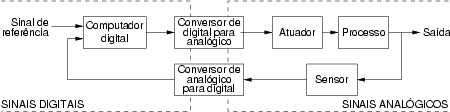
\includegraphics{textuais/04-figuras/figuras/bigbitmap}
%\caption{Figura \emph{pixel}-a-\emph{pixel} grande em tamanho natural}
%\label{Fig:bigbitmap}
%\vspace{6mm}
%\includegraphics[scale=0.5]{textuais/04-figuras/figuras/bigvetorial}
%\caption{Figura vetorial grande em tamanho reduzido}
%\label{Fig:bigvetorialreduzida}
%\vspace{6mm}
%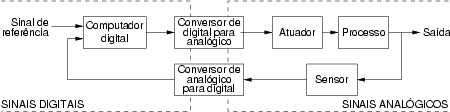
\includegraphics[scale=0.5]{textuais/04-figuras/figuras/bigbitmap}
%\caption{Figura \emph{pixel}-a-\emph{pixel} grande em tamanho reduzido}
%\label{Fig:bigbitmapreduzida}
%\end{center} \end{figure}
%
%\begin{figure}[htbp!] \begin{center}
%\includegraphics{textuais/04-figuras/figuras/smallvetorial}
%\caption{Figura vetorial pequena em tamanho natural}
%\label{Fig:smallvetorial}
%\vspace{6mm}
%\includegraphics{textuais/04-figuras/figuras/smallbitmap}
%\caption{Figura \emph{pixel}-a-\emph{pixel} pequena em tamanho natural}
%\label{Fig:smallbitmap}
%\vspace{6mm}
%\includegraphics[width=\linewidth]{textuais/04-figuras/figuras/smallvetorial}
%\caption{Figura vetorial pequena em tamanho ampliado}
%\label{Fig:smallvetorialampliada}
%\vspace{6mm}
%\includegraphics[width=\linewidth]{textuais/04-figuras/figuras/smallbitmap}
%\caption{Figura \emph{pixel}-a-\emph{pixel} pequena em tamanho ampliado}
%\label{Fig:smallbitmapampliada}
%\end{center} \end{figure}
%
%Nota-se que no formato vetorial as
%linhas mantêm a espessura mesmo quando se fazem
%ampliações ou reduções. Já no formato de \emph{pixels}
%as linhas ficam mais claras (cinzas, ao invés de pretas) após as
%reduções e mais grossas após as ampliações, além de uma perda geral
%de definição da imagem.
%
%\section{Ferramentas para desenhos e esquemas}
%\label{Sec:desenhos}
%
%Existem diversas ferramentas para fazer desenhos, mas muitas delas
%apenas salvam a figura gerada em formatos \emph{pixel}-a-\emph{pixel}.
%No Unix, pode-se utilizar o \texttt{xfig}, que exporta imagens em
%muitos formatos, inclusive nos vetoriais (PDF e EPS). Os diagramas das
%figuras \ref{Fig:bigvetorial} a \ref{Fig:smallbitmapampliada} foram
%desenhados e exportados no \texttt{xfig}. O arquivo fonte
%correspondente é o \texttt{diagrama.fig}, no diretório
%\texttt{figuras}.
%
%A possibilidade de salvar figuras em modo vetorial impõe que alguns
%recursos para desenho de imagens não sejam oferecidos. Um deles é o
%desenho a mão-livre, já que seria impossível descrever a curva obtida
%em termos de figuras geométricas básicas. Outro recurso inexistente é
%o de preencher uma região com uma determinada cor. Esta última
%limitação muitas vezes pode ser contornada utilizando-se a noção de
%profundidade.  Por exemplo, para desenhar uma figura vazado e
%preenchido de azul, pode-se desenhar a figura externa preenchido de
%azul sobre o qual se desenha a figura interna preenchido de branco,
%como mostram os exemplos da figura~\ref{Fig:circulo}.
%
%\begin{figure}[htb] \begin{center}
%\includegraphics{textuais/04-figuras/figuras/circulo}
%\caption{Preenchimento de figuras utilizando diferentes profundidades}
%\label{Fig:circulo}
%\end{center} \end{figure}
%
%A noção de profundidade no \texttt{xfig} foi exaustivamente utilizada
%para desenhar os símbolos da UFRN e do PPgEE que podem ser vistos na
%página de rosto deste documento. Os arquivos \texttt{xfig}
%correspondentes são \texttt{UFRN.fig} e \texttt{PPgEE.fig}. Ela também
%pode ser utilizada para mesclar imagens com figuras sintéticas, como
%na figura \ref{Fig:pensador} (veja arquivo \texttt{figuras/pensador.fig}).
%
%\begin{figure}[htb] \begin{center}
%\includegraphics{textuais/04-figuras/figuras/pensador}
%\caption{Imagem mesclada com elementos sintéticos}
%\label{Fig:pensador}
%\end{center} \end{figure}
%
%Outra possibilidade oferecida pelo \texttt{xfig} é a inclusão de comandos
%\LaTeX\ dentro da figura. Para utilizar este recurso,
%marque no \texttt{xfig} os textos que devem ser interpretados como
%comandos \LaTeX\ com o \emph{flag} \texttt{special} e exporte a figura
%no modo \emph{Combinado PS/Latex} ou \emph{Combinado PDF/Latex}. Veja
%um exemplo na figura \ref{Fig:combinado}; note que o arquivo é incluído com
%\verb|\input{}| e não com \verb|\includegraphics{}|.
%
%% Note que foi redefinido um comando aqui no texto para ser incluído
%% na figura. Isto é para evitar digitação de expressões LaTeX muito
%% grandes dentro do xfig
%\newcommand{\formulagrande}{$\frac{G_3G_4}{1-G_3G_4H_1}$}
%\begin{figure}[htb] \begin{center}
%%\input{figuras/combinado.pstex_t} % Se usar latex
%\input{textuais/04-figuras/figuras/combinado.pdftex_t} % Se usar pdflatex
%\caption{Figura incluindo comandos \LaTeX}
%\label{Fig:combinado}
%\end{center} \end{figure}
%
%\section{Ferramentas para gráficos}
%\label{Sec:graficos}
%
%Gráficos devem ser gerados com aplicativos capazes de exportar o
%resultado nos formatos EPS ou PDF, preferencialmente em formato
%vetorial. Os conhecidos programas \emph{Scilab} e \emph{Matlab} têm
%esta capacidade. Se você deseja algo mais simples, a ferramenta
%\textit{GNUplot} é uma das mais utilizadas no Unix para a geração de
%gráficos de funções matemáticas.
%
%Uma vez gerados, gráficos são inseridos no texto tal como figuras. A
%figura~\ref{fig:grafico} apresenta um gráfico gerado através do
%comando de linha \texttt{gnuplot grafico.gnuplot}. Este arquivo
%\texttt{grafico.gnuplot}, que contém uma série de comandos do
%\textit{GNUplot}, está no diretório \texttt{figuras}.
%
%\begin{figure}[htbp]
%\centering
%\includegraphics{textuais/04-figuras/figuras/grafico}
%\caption{Exemplo de gráfico de funções matemáticas}
%\label{fig:grafico}
%\end{figure}
%
%\section{Conclusões}
%
%Ferramentas de desenho capazes de gerar a saída em formato vetorial
%são mais difíceis de usar e parecem ser dotadas de menos recursos do
%que outras que só exportam seus resultados como imagens de
%\emph{pixels}.  Isto se deve à necessidade de descrever todos os
%elementos da imagem sob a forma de primitivas parametrizáveis para
%permitir que elas sejam escaláveis à vontade e exportáveis para
%qualquer formato desejado.
%
%Entretanto, a qualidade visual das figuras obtidas e a sua
%reusabilidade é muito maior. A comparação é aproximadamente a mesma
%que a entre textos produzidos em \LaTeX\ e em editores gráficos. Desta
%forma, na medida do possível, tente conjugar a escrita do documento
%\LaTeX\ com a utilização de alguma ferramenta de desenho vetorial.
%
%% LocalWords:  editadas PS

%%
%% Capítulo 5: Conclusões
%%

\mychapter{Conclusão}
\label{Cap:Conclusao}

O capítulo final depende do tipo de documento. Nas propostas de tema
deve ser apresentado de forma clara e sucinta o assunto a ser
desenvolvido e o cronograma de execução do trabalho. Nos trabalhos de conclusão de curso (TCC) deve ser ressaltadas as principais contribuições do
trabalho e as suas limitações.

As contribuições devem evitar as adjetivações e julgamentos de valor.
Quanto às limitações, não tenha medo de as apresentar: é muito mais
reconhecido um autor que apresenta os casos em que sua proposta não se
aplica do que outro que parece não ter consciência deles.

Escreva (com outras palavras) o que foi realizado e como foi realizado, o que o trabalho descrito no artigo conseguiu melhorar e qual a sua relevância, e quais são as vantagens e limitações da proposta que o TCC apresenta. Apresente também eventuais aplicações dos resultados obtidos (ou da metodologia, técnica, produto) e ideias de trabalhos futuro que possam melhorar o seu (não apenas apresente, mas indique como pode ser feito).

%\section{Encadernação}
%
%As propostas de tema e as versões iniciais das teses e dissertações
%são impressas em lado único da folha e em espaçamento um e meio. Para
%a encadernação, usa-se geralmente um método simples, tal como espiral
%na lateral das folhas e capa plástica transparente. O número de cópias
%é igual ao número de membros da banca e pelo menos mais uma (para o
%aluno).
%
%As versões finais das teses e dissertações são impressas em frente e
%verso e em espaçamento simples. O número mínimo de cópias é o seguinte:
%\begin{itemize}
%\item 3 cópias para o PPgEEC e a UFRN.
%\item 1 cópia para cada examinador externo que participou da banca.
%\item ao menos 1 cópia para o aluno (não obrigatória).
%\item 1 cópia para o orientador (por cortesia, não obrigatória)
%\end{itemize}
%
%Para a encadernação, deve-se adotar uma capa rígida de cor azul para
%as dissertações de mestrado e de cor preta para as teses de doutorado,
%ambas com letras douradas. Na capa deve constar o título do
%trabalho, o autor e o ano da defesa. Se possível, a mesma informação
%deve ser repetida na lombada do livro.
%
%Para as versões finais, também se exige uma cópia eletrônica (formato
%PDF) do texto, bem como outros dados. Maiores informações podem ser
%obtidas na página do PPgEEC: \url{http://www.ppgeec.ufrn.br/}

\section{Etapas de Homologação do Título}

A seguir apresentamos as etapas necessárias para a apresentação do TCC à banca de avaliação e o seu depósito na biblioteca.

\begin{enumerate}
	\item Após a conclusão do trabalho, o orientador deverá informar ao professor responsável pela disciplina de Trabalho de Conclusão de Curso, os membros que irão compor a banca examinadora e combinar o agendamento do horário e o local da apresentação;
	\item O professor responsável pela disciplina de Trabalho de Conclusão de Curso dará publicidade à apresentação e organizará em processo SEI, a Ata de Apresentação, a Avaliação da Banca e as Declarações de Participação de Banca de Defesa de TCC para os membros da banca examinadora;
	\item Após a apresentação e as correções que se fizerem necessárias ao TCC, o estudante deverá solicitar via processo SEI, destinado à coordenação do curso, o registro e a disponibilização do seu TCC no acervo da biblioteca. O estudante deverá anexar ao processo os seguintes documentos:
	\begin{itemize}
		\item Declaração do Orientador do TCC seguindo o modelo que consta no apêndice deste documento;
		\item Ata de Defesa de TCC que consta no processo SEI criado pelo professor responsável pela disciplina de TCC;
		\item Avaliação da Banca Examinadora que consta no processo SEI criado pelo professor responsável pela disciplina de TCC;
		\item O Trabalho de Conclusão de Curso em PDF;
		\item Termo de Autorização do Autor preenchido disponível no Anexo A.
	\end{itemize}
	\item Se o processo estiver corretamente instruído, a coordenação do curso encaminhará a solicitação à Biblioteca.
\end{enumerate}

\section{Para saber mais}

Procure no Google, ora! Brincadeiras a parte, existem inúmeros
tutoriais sobre \LaTeX\ na rede que podem dar maiores informações
sobre o aplicativo. Para conhecer os pacotes disponíveis, uma opção é
o livro \emph{The \LaTeX\ Companion} \cite{LATEX04}, popularmente
conhecido como o ``livro do cachorro''. Outras informações sobre
redação técnica e normas para confecção de teses e dissertações podem
ser encontradas em livros de Metodologia Científica.


% Referências bibliogáficas (geradas automaticamente)
\phantomsection
\addcontentsline{toc}{chapter}{Referências bibliográficas}
\bibliography{bibliografia/bibliografia}

\begin{appendices}
\appendix
%%
%% Apêndice
%%

\mychapter{Tabelas Completas}
\label{Cap:apendiceA}

Todas as tabelas que são grandes demais para serem incluídas no texto estão apresentadas neste apêndice.

\section{Tabela de requisitos funcionais}

\begin{longtable}{| p{.15\textwidth} | p{.40\textwidth} | p{.15\textwidth} |  p{.15\textwidth} |} \hline
\textbf{Identificador} & 
\textbf{Descrição} & 
\textbf{Prioridade} & 
\textbf{Requisitos Relacionados} \\ \hline
RF01 & 
O sistema deve permitir que os usuários modelarem a dinâmica dos sensores presentes em uma planta industrial. & 
Alta & 
RF02 \\ \hline
RF02 &
Os usuários devem ser capazes de alimentar o sistema com os dados gerados pelos sensores. &
Alta &
RF01 \\ \hline
RF03 & 
O sistema deve oferecer uma interface de usuário intuitiva e acessível. 
& Média 
& - \\ \hline
RF04 & 
O sistema deve realizar cálculos de reconciliação de dados de forma ágil e rápida. & 
Alta & 
RF01, RF02 \\ \hline
RF05 & 
O sistema deve garantir a compatibilidade de dados, mesmo com formatos heterogêneos. & 
Alta & 
RF01, RF02, RF03 \\ \hline
RF06 & 
Os usuários devem poder exportar os resultados da reconciliação de dados para diferentes formatos de arquivo. & 
Média &
RF01, RF02, RF03, RF04, RF05 \\ \hline
RF07 & 
O sistema deve permitir aos usuários configurar alertas para notificar sobre eventos importantes relacionados aos dados dos sensores. & 
Alta & 
RF01, RF02 \\ \hline
RF08 
& O sistema deve fornecer funcionalidades de visualização de dados em tempo real, incluindo gráficos e relatórios personalizáveis. &
Alta &
RF02, RF05 \\ \hline
RF09 & 
O sistema deve permitir a integração com outros sistemas de monitoramento industrial, facilitando a troca de dados e informações. & 
Alta & 
RF05, RF06 \\ \hline
\caption{Tabela completa dos requisitos funcionais do \textit{software}.}
\label{tab:apendice_req_funcionais}
\end{longtable}

\section{Tabela de requisitos não funcionais}

\begin{longtable}
{| p{.15\textwidth} | p{.55\textwidth} | p{.15\textwidth} |} 
    \hline
    \textbf{Identificador} & \textbf{Descrição} & \textbf{Prioridade} \\
    \hline
    RNF01 & O sistema deve ser altamente escalável para lidar com um grande volume de dados de sensores. & Alta \\
    \hline
    RNF02 & A segurança dos dados deve ser uma prioridade, garantindo proteção contra acesso não autorizado e manipulação indevida. & Alta \\
    \hline
    RNF03 & O desempenho do sistema deve ser otimizado para garantir tempos de resposta rápidos, mesmo em momentos de pico de uso. & Alta \\
    \hline
    RNF04 & O sistema deve ser facilmente configurável e customizável para atender às necessidades específicas de diferentes ambientes industriais. & Média \\
    \hline
    RNF05 & A manutenibilidade do sistema deve ser uma consideração fundamental, facilitando atualizações, correções de bugs e modificações futuras. & Média \\
    \hline
    RNF06 & A usabilidade do sistema deve ser intuitiva, permitindo uma curva de aprendizado mínima para os usuários. & Média \\
    \hline
    RNF07 & O sistema deve ser compatível com diferentes navegadores, garantindo sua acessibilidade em uma variedade de ambientes de implantação. & Alta \\
    \hline
    RNF8 & O sistema deve estar em conformidade com regulamentações de privacidade de dados, como GDPR, garantindo o tratamento adequado e a proteção das informações pessoais dos usuários. & Alta \\
    \hline
    RNF9 & A tolerância a falhas do sistema deve ser implementada, garantindo a continuidade das operações mesmo em caso de falhas de componentes individuais. & Alta \\
    \hline
    RNF10 & O tempo de resposta do sistema deve ser consistente e previsível, independentemente da carga de trabalho ou do número de usuários simultâneos. & Média \\
    \hline
\caption{Tabela de Requisitos Não Funcionais} % needs to go inside longtable environment
\label{tab:apendice_req__naofuncionais}
\end{longtable}
\end{appendices}

\renewcommand{\appendixname}{Anexo}
\begin{appendices}
\appendix
% %%
% %% Anexo
% %%

% \mychapter{Termo de Autorização do Autor}
% \label{Cap:anexo}

% A principal diferença entre anexo e apêndice é que os apêndices são textos criados pelo próprio autor para complementar sua argumentação, enquanto os anexos são documentos criados por terceiros e usados pelo autor.

% Tanto o apêndice quanto o anexo devem estar presentes no sumário dos trabalhos científicos. Os apêndices devem aparecer depois das referências e os anexos depois dos apêndices.

% 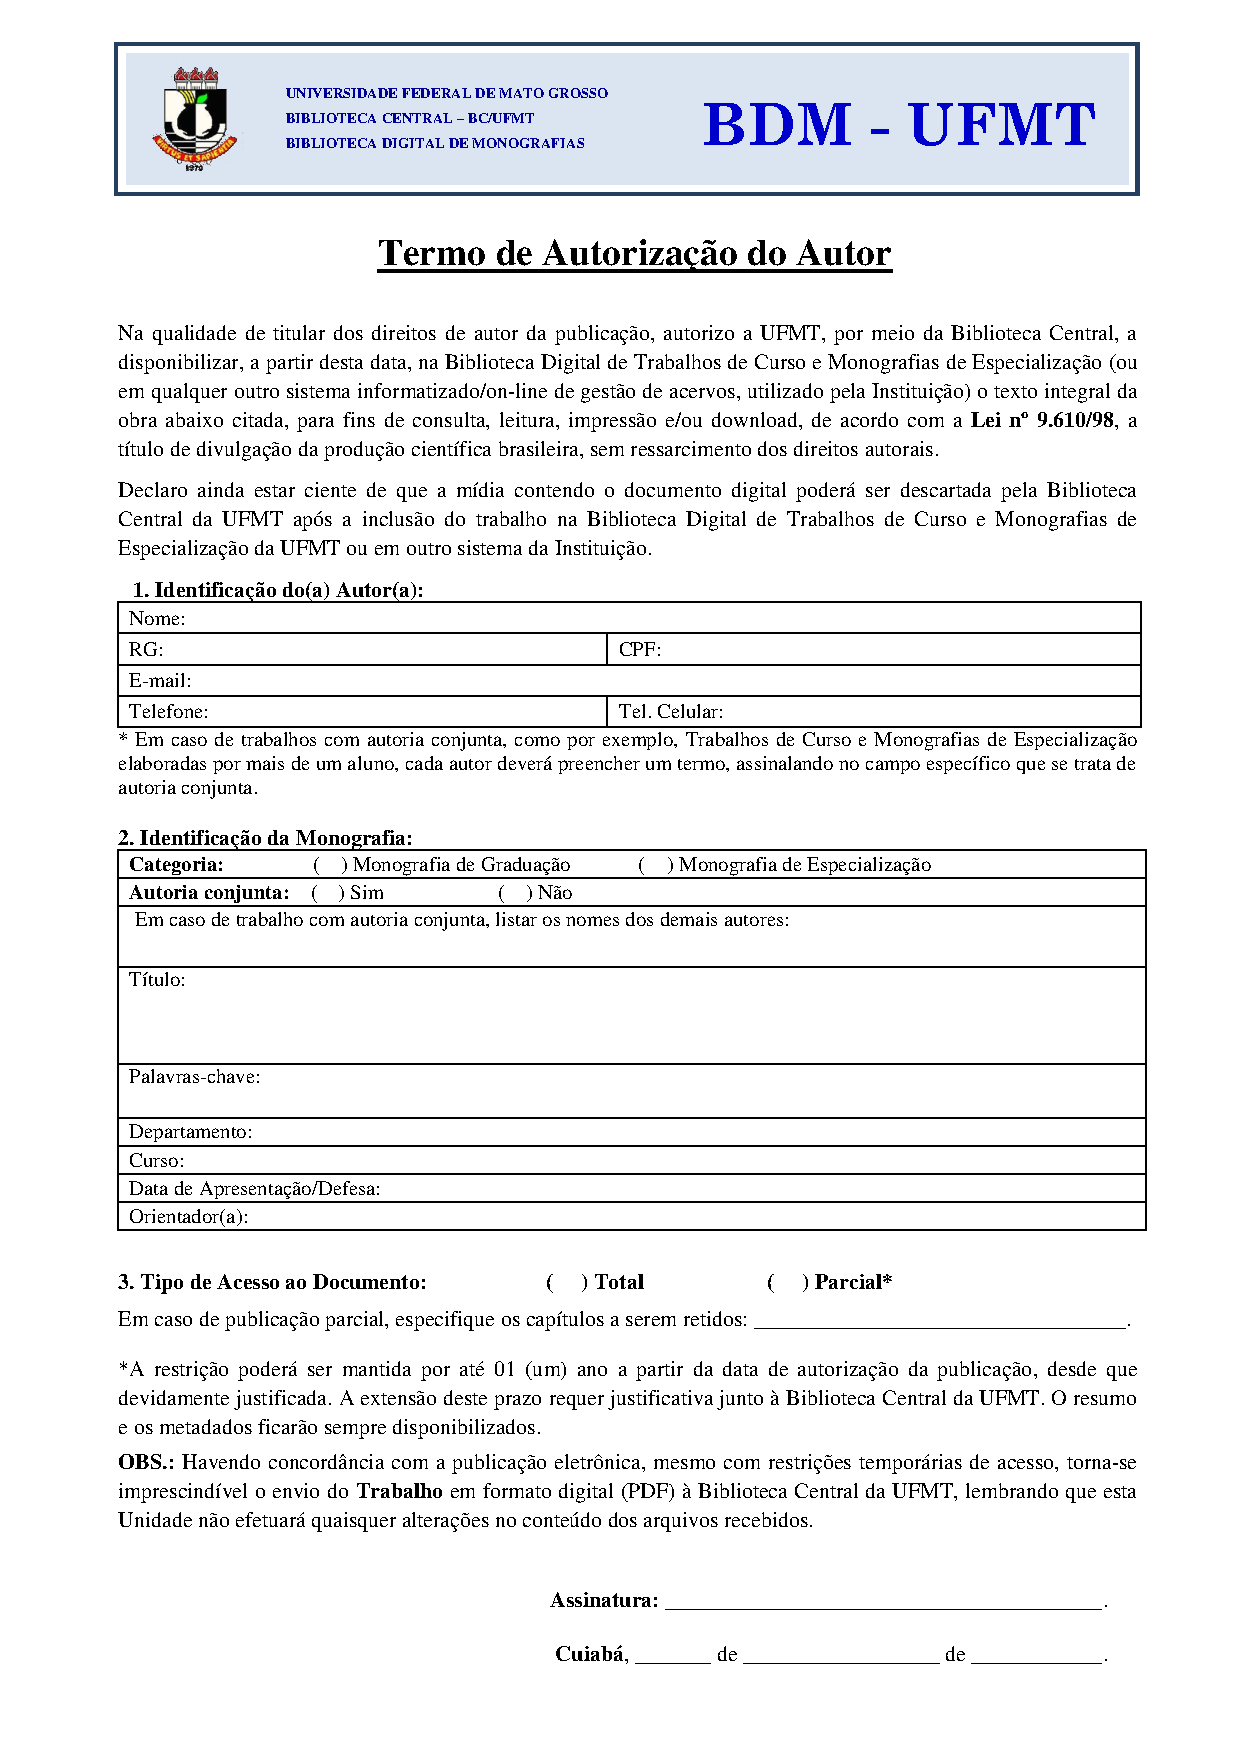
\includepdf[pages=-]{textuais/anexo/termo_de_autorizacao.pdf}

\end{appendices}

\end{document}
